\documentclass[11pt]{article}
\usepackage{multirow}
\usepackage{hyperref}
\usepackage{xr}
\usepackage[export]{adjustbox}
\usepackage{float}
\usepackage[caption = false]{subfig}
\usepackage{graphicx}
\usepackage{hyperref}
\usepackage{units}
%\usepackage[small, bf]{caption}
\usepackage[numbers,sort&compress]{natbib}
\usepackage{color}
\usepackage{amssymb, amsmath}
%\usepackage{epstopdf}
%\usepackage{ulem}
\usepackage{verbatim}
\usepackage{amsfonts}
%\usepackage{subfloat}
\usepackage{subfig}
%\usepackage{multirow}
\usepackage{authblk}
%\usepackage{array}
%\usepackage{footmisc}
%\usepackage{tabularx}
%\usepackage{sidecap}
\usepackage{setspace}
\usepackage{graphicx}
%\usepackage{caption}
%\usepackage{subcaption}
\usepackage[normalem]{ulem}
\usepackage[margin=1in]{geometry}
\usepackage[usenames,dvipsnames,table,xcdraw]{xcolor}
%\usepackage{rotating}
\renewcommand\Affilfont{\small}
\newcommand{\ignore}[1]{}
\graphicspath{{figures/}}

\newcommand{\doubleline}[2][c]{%
	\begin{tabular}[#1]{@{}c@{}}#2\end{tabular}}

\newtheorem{theorem}{Theorem}
%\newtheorem{acknowledgement}[theorem]{Acknowledgement}
%\newtheorem{algorithm}[theorem]{Algorithm}
% \newtheorem{axiom}[theorem]{Axiom}
%\newtheorem{case}[theorem]{Case}
%\newtheorem{claim}[theorem]{Claim}
%\newtheorem{conclusion}[theorem]{Conclusion}
%\newtheorem{condition}[theorem]{Condition}
%\newtheorem{conjecture}[theorem]{Conjecture}
%\newtheorem{corollary}[theorem]{Corollary}
%\newtheorem{criterion}[theorem]{Criterion}
%\newtheorem{definition}[theorem]{Definition}
%\newtheorem{example}[theorem]{Example}
%\newtheorem{exercise}[theorem]{Exercise}
\newtheorem{lemma}[theorem]{Lemma}
%\newtheorem{notation}[theorem]{Notation}
%\newtheorem{problem}[theorem]{Problem}
%\newtheorem{proposition}[theorem]{Proposition}
%\newtheorem{remark}[theorem]{Remark}
%\newtheorem{solution}[theorem]{Solution}
%\newtheorem{summary}[theorem]{Summary}
\newenvironment{proof}[1][Proof]{\textbf{#1.} }{\ \rule{0.5em}{0.5em}}



\newenvironment{packed_enum}{
\begin{enumerate}
  \setlength{\itemsep}{1pt}
  \setlength{\parskip}{0pt}
  \setlength{\parsep}{0pt}
}{\end{enumerate}}
\newenvironment{packed_itemize}{
\begin{itemize}
  \setlength{\itemsep}{1pt}
  \setlength{\parskip}{0pt}
  \setlength{\parsep}{0pt}
}{\end{itemize}}
\newenvironment{packed_desc}{
\begin{description}
  \setlength{\itemsep}{1pt}
  \setlength{\parskip}{0pt}
  \setlength{\parsep}{0pt}
}{\end{description}}

%%\def\glenn#1{{\textcolor{red}{GT note: #1}}}
\def\VB#1{{\textcolor{blue}{VB note: #1}}}
\def\SM#1{{\textcolor{orange}{SM note: #1}}}
\def\ali#1{{\textcolor{JungleGreen}{Ali note: #1}}}

\def\figfmt{png}
\def\figsuffix{_reduced_size}
%\def\figsuffix{}
\def\MDDAF{\text{MDDAF}}
\def\DAF{\text{DAF}}

\def\dHAF{\text{-HAF}}
\def\HAF{\text{HAF}}
\def\HAFpeak{\text{HAF-peak}}
\def\HAFtrough{\text{HAF-trough}}
\def\HAFneutral{\text{HAF}_{\text{neutral}}}
\def\TMRCA{T_{\text{MRCA}}}

\def\all{\,\text{all}}
\def\car{\,\text{car}}
\def\ncar{\,\text{non}}

\def\MRCAall{\text{MRCA}^{\text{all}}}
\def\MRCAcar{\text{MRCA}^{\text{car}}}
\def\MRCAnon{\text{MRCA}^{\text{non}}}

\def\AlleleFreq{\text{AlleleFreq}}
\def\AlleleFreqNeutral{\text{AlleleFreq}_{\text{neutral}}}

\def\SAFE{\text{SAFE}}
\def\iSAFE{\text{iSAFE}}

\def\vecbold#1{{\bf#1}}
\def\mathbi#1{\textbf{\em #1}}

%\doublespacing % 2 line spacing
\onehalfspacing % 1.5 line spacing

\newcommand{\algoname}{\ensuremath{\text{PreCIOSS}}}


%%%%%%%%%%%%
\makeatletter
\renewcommand\section{\@startsection {section}{1}{\z@}%                                                                                                         
                                   {-3.2ex \@plus -1ex \@minus -.2ex}%                                                                                        
                                   {2.0ex \@plus.2ex}%                                                                                                        
                                   {\normalfont\Large\bfseries}}
\renewcommand\subsection{\@startsection{subsection}{2}{\z@}%                                                                                                    
                                     {-2.95ex\@plus -1ex \@minus -.2ex}%                                                                                      
                                     {1.2ex \@plus .2ex}%                                                                                                     
                                     {\normalfont\large\bfseries}}
\renewcommand\subsubsection{\@startsection{subsubsection}{3}{\z@}%                                                                                              
                                     {-2.95ex\@plus -1ex \@minus -.2ex}%                                                                                      
                                     {1.2ex \@plus .2ex}%                                                                                                     
                                     {\normalfont\normalsize\bfseries}}
\renewcommand\paragraph{\@startsection{paragraph}{4}{\z@}%                                                                                                      
                                    {1.55ex \@plus1ex \@minus.2ex}%                                                                                           
                                    {-.7em}%                                                                                                                   
                                    {\normalfont\normalsize\bfseries}}


%\externaldocument{supplement}

\topmargin 0.0cm
\oddsidemargin 0.2cm
\textwidth 16cm 
\textheight 21cm
\footskip 1.0cm


%The next command sets up an environment for the abstract to your paper.

\newenvironment{sciabstract}{%
\begin{quote} \bf}
{\end{quote}}
\def\VB#1{{\textcolor{blue}{VB note: #1}}}


% If your reference list includes text notes as well as references,
% include the following line; otherwise, comment it out.

\renewcommand\refname{References and Notes}

% The following lines set up an environment for the last note in the
% reference list, which commonly includes acknowledgments of funding,
% help, etc.  It's intended for users of BibTeX or the {thebibliography}
% environment.  Users who are hand-coding their references at the end
% using a list environment such as {enumerate} can simply add another
% item at the end, and it will be numbered automatically.

\newcounter{lastnote}
\newenvironment{scilastnote}{%
\setcounter{lastnote}{\value{enumiv}}%
\addtocounter{lastnote}{+1}%
\begin{list}%
{\arabic{lastnote}.}
{\setlength{\leftmargin}{.22in}}
{\setlength{\labelsep}{.5em}}}
{\end{list}}


% Include your paper's title here

\title{ViFi: Viral integration and mRNA fusion identification} 


% Place the author information here.  Please hand-code the contact
% information and notecalls; do *not* use \footnote commands.  Let the
% author contact information appear immediately below the author names
% as shown.  We would also prefer that you don't change the type-size
% settings shown here.

\author
{Nam-phuong Nguyen$^{1}$, Viraj Deshpande$^{1}$, 
Jens Luebeck$^{2}$, Paul Mischel$^{3}$, and Vineet Bafna$^{1\ast}$\\
\normalsize{$^{1}$Computer Science and Engineering, University of California,}\\
\normalsize{San Diego, La Jolla, 92093, USA.,}\\
\normalsize{$^{2}$Bioinformatics and Systems Biology Program, University of California,}\\
\normalsize{San Diego, La Jolla, 92093, USA.,}\\
\normalsize{$^{3}$Department of Pathology, University of California,}\\
\normalsize{San Diego, La Jolla, 92093, USA.,}\\
\normalsize{$^\ast$To whom correspondence should be addressed; E-mail:  vbafna@eng.ucsd.edu.}
}

% Include the date command, but leave its argument blank.

\date{}

%%%%%%%%%%%%%%%%% END OF PREAMBLE %%%%%%%%%%%%%%%%



\begin{document} 

% Double-space the manuscript.

\baselineskip24pt

% Make the title.

\maketitle 

% Place your abstract within the special {sciabstract} environment.

\begin{sciabstract}
An estimated 10\% of new human cancer cases are caused by oncoviruses, with more than 67\% of the cases occurring in developing countries.  In cancers such as cervical cancer and hepatocellular carcinoma, the integration of the viral genome into the host cell's genome is an important factor tumorigenesis.  Standard approaches to viral integration detection is identifying paired-end reads mapping to both the human and viral references.  However, read-based reference mapping has difficulty identifying integration sites from rapidly evolving viruses or from novel virus strains.  We present ViFi, a viral integration detection tool which uses both reference-based read mapping and a phylogenetic-based approach to identify viral reads.  Key to this framework is the use of profile Hidden Markov models to represent the viral family of interest, allowing the detection of highly mutated or novel  sequences belonging to a viral family.  In addition, ViFi uses mappability scores to reduce false positive detections.  ViFi can be run on WGS and RNA-seq data, allowing for both the detection of integration sites and fusion transcripts.  We compare Viral-HMM to VERSE and ViralFusionSeq on both simulated NGS data and real biological data with experimentally verified integration sites.  Our results show that ViFi is more sensitive in detecting integration sites and has a lower false positive detection rate.
\end{sciabstract}

\section*{Introduction}
Infection agents such as viruses, bacteria, and parasites are recognized as major factors in cancer etiology.  Plummer et al. (2016) reported that infection agents can be attributed to 15\% of all new cancer cases in 2012, of which 64\% can be attributed to oncoviruses.  These oncoviruses include the Human papillomavirus (HPV) which accounts for almost 100\% of all cervical cancers and half of all infection-attributed cancers in women, and Hepatitis B virus (HBV) and Hepatitis C virus (HCV) which account for 74\% of all liver cancer cases~\cite{Plummer2016}.  Both HPV and HBV are DNA viruses and have mechanisms for integrating directly into the host genome, and genomic surveys of HPV- and HBV-infected tumor samples show the same integration site throughout the sample, suggesting that integration occurred before clonal expansion of the tumor sample.  This observation suggests that integration may lead to cellular proliferation and cancer formation~\cite{Moore2010}.

With the advent of Next Generation Sequencing (NGS) technology, human genomes can now be sequenced with high coverage and high sequencing depth thus making it more feasible to accurately identify the location of viral integrations within the human genome.  Studies of the impact of viral integration on tumorigenesis have found evidence of recurrent genomic hotspots in both HBV-related hepatocellular carcinoma (HCC; ~\cite{Ding2012, Khoury2013}) and HPV-related cervical cancers~\cite{Schmitz2012}.  In these studies recurrent integrations were often found in or near known oncogenes such as TERT, MYC, and MLL4, suggesting that integration occurs randomly across the genomic, however over the course of tumor formation progression, integrations in key genomic regions may provide a selective advantage for the host cells, resulting in recurrent integration sites across different samples.  The majority of HPV and HCC tumors, however, do not contain recurrent integration sites.  Thus, focusing on just recurrent integration sites may provide an incomplete story of the role of viral integration on tumor formation.  

Crucial to untangling the role of integration on tumor formation is the ability to accurately detect integrated viruses from NGS data.  Many pipelines have been developed recently for the detection of viral integration from paired-end Illumina data (VirusSeq~\cite{Chen2013}, VirusFinder~\cite{Wang2013}, ViralFusionSeq~\cite{Li2013} in 2013; VERSE~\cite{Wang2015}, Virus-Clip~\cite{Ho2015}, and Vy-PER~\cite{Forster2015} in 2015).  While each pipeline varies in how detection is performed, the overarching theme is similar: identify single end or paired-end reads that map to both the human and viral reference genome.  However, the task of identifying viral integrations from NGS technology is still challenging.  For example, the integrations from ~\cite{Hu2015} have been challenged as false positives integrations as a result of PCR sequencing artifacts~\cite{Dyer2015}.  Indeed, one of the large problems with viral integration detection lies in separating out true integrations from false positives integrations, which often can result from shared repeat regions between human and viral genomes~\cite{Forster2015}.  

Here, we present \textbf{V}iral \textbf{I}ntegration and \textbf{F}usion \textbf{I}dentification (ViFi), a new tool for detecting viral integrations from WGS data and human-virus fusion mRNA from RNASeq data (Fig.~\ref{flowchart}).  Unlike other viral integration detection pipelines that use reference-based alignment mapping for identifying viral reads, ViFi uses a combination of reference-based alignment mapping and evolutionary models of the viral families of interest to identify viral reads.  In addition, ViFi incorporates the mappability scores to reduce false positive detections.  The end result is a tool that can accurately detect viral integrations with high precision and recall, even when the viruses are highly mutated or are not found in the reference Papillomavirus genomes.  

We show a comparison ViFi to competing tools, VERSE and ViralFusionSeq, on both simulated and biological datasets with experimentally verified integrations.  These datasets include simulated WGS of genomes containing integrated HPV (HPV-SIM), WGS from HCC samples taken from patients with HBV~\cite{Sung2012} (HCC-WGS), RNA-seq datasets from HCC cell lines infected with HBV~\cite{Lau2014} (HCC-RNA).  We also compared the fusion mRNA sequences found by ViFi and VERSE to those from another study on fusion human-viral mRNA transcripts~\cite{Tang2013} on tumor cervical samples taken from the The Cancer Genome Atlas (TCGA-CESC).  Finally, we perform a comprehensive analysis on the impact of HPV integration on transcription expression using matched paired WGS and RNA-seq data from the TCGA-CESC datasets.  

\section*{Results}

\paragraph{\textbf{Comparison on simulated datasets.}}  We simulated WGS datasets with integrated viruses, exploring the impact of viral strain diversity and number of integrations on detection accuracy and computational running time.  The integrated viruses included three HPV16 strains simulated with either low, medium, or high rates of substitution mutation, and one papillomavirus (AgPV1) that is not included the reference PV database to simulate detection of a novel virus.  The number of integrations varied from 25, 100, 500, and 1000.  For each model condition (parameterized by the integrated virus and number of integrations), we generated five replicate WGS datasets at 25x coverage (approximately 50 GB of data per dataset) for a total of 16 model conditions and 80 datasets.  

We ran ViFi, either with using only the reference-based mapping or using the combination of reference-based mapping and eHMMs, VERSE, and ViralFusionSeq on the simulated datasets (Fig.~\ref{sim_results}.  All methods were run on a dedicated compute node and given 48 hours to complete.  Only ViFi was able to complete within the allotted time on all datasets. VERSE completed only on datasets with less than \textbf{XXX [NOTE:  Need to wait for runs with 100, 500 integrations to complete]} integrations, while ViralFusionSeq failed to complete on any of the datasets.  Due to the computational cost of running ViralFusionSeq, we excluded it from the remainder of this study.

Both ViFi (both with and without HMMs) and VERSE have high precision and recall on the easier datasets (95-99\% similarity with HPV16).  However, when the integrated virus has only 90\% similarity to HPV16, VERSE's precision and recall drops by one half.  ViFi, on the other hand, is still able to accurately detect the highly mutated simulated HPV16 sequence.  On the dataset that contains the novel AgPV1 sequence, only ViFi with the HMMs is able to accurately detect integration events (88\% recall and 93\% precision).  ViFi without the HMMs is only able to detect 20\% of the integrations, but with high precision.  VERSE is unable to detect any integration events.  

Interestingly, VERSE takes significantly longer when it detects more integrations.  When no integrations are detected, it takes roughly 6 hours to complete, however, this time jumps by two to three hours when it detects 20 or more integrations.  Thus, VERSE fails to complete on any dataset with more than \textbf{XXX} integrations.  ViFi, on the other hand, had an average increase of running time of 32 minutes when increasing the number of simulated viral integrations from 25 to 1000 integrations, without any loss of recall or precision.  As some cervical cancer samples can have up to 100 to 600 HPV integration events~\cite{Hu2015}, it is vital that integration pipelines are able to run efficiently on samples with many integrations.\textbf{NOTE:  Simulations being run for 100 and 500 integrations, will be able to better discuss scaling once complete.}

%We ran ViFi, either with using only the reference-based mapping or using the combination of reference-based mapping and eHMMs, VERSE, and ViralFusionSeq on the simulated datasets that contained 25 viral integrations per dataset (Fig.~\ref{sim_results}).  %All methods were run on a dedicated compute node with 24 CPUs and given 48 hours to complete.  Only ViFi and VERSE completed within the allotted time; ViralFusionSeq failed to complete on any of the datasets.  ViFi required an average wall clock running time of 7 hours and 30 minutes (minimum of hours 13 minutes to maximum of 8 hours and 2 minutes).  The impact of using HMMs had minimal impact on the running time of ViFi (average increase of 14 seconds).  VERSE required an average of 8 hours and 19 minutes to complete per dataset (minimum of 6 hours and 1 minute to a maximum of 9 hours and 19 minutes).  Due to ViralFusionSeq being unable to complete on these datasets, we exclude ViralFusionSeq from the remainder of our comparison study.

\begin{figure}[htpb]
  \centering
  \subfloat[Precision-recall on simulated datasets.]{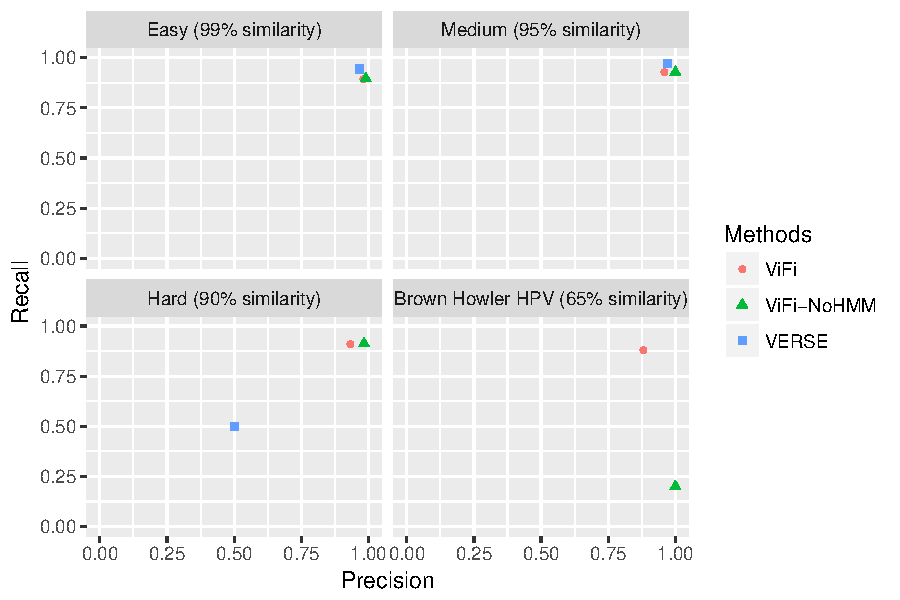
\includegraphics[width=4in,frame]{{results/simulation.main}.pdf}}\\
  \subfloat[Running time on simulated datasets.]{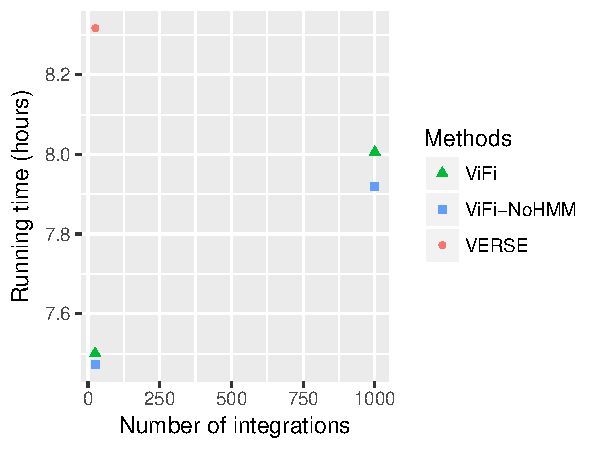
\includegraphics[width= 4in,frame]{{results/running}.pdf}}  
\caption[Results on simulated datasets.]
{\label{sim_results}  {\bf Results on simulated datasets.}  We report a) the recall and precision for four different model conditions with 25 simulated viral integrations, and b) wall clock running time for the easy model HPV16 model condition.  We show results for when we include the usage of the  ensemble of HMMs in detecting viral reads (Default) and when we exclude the usage of the ensemble of HMMs (Default-NoHMMs).  The first three model conditions (easy, medium, and hard) vary the percent similarity of simulated HPV16 genomes to the reference HPV16 genome, with five replicates per simulation.  The last model condition uses Alouatta guariba papillomavirus 1 (AgPV1), a PV genome not included in the set of viral genomes to simulate detection of a novel HPV virus.  AgPV1 is 44\% similar to HPV16.  VERSE failed to detect any viruses on the AgPV1 model condition.  All datasets were simulated with 25x coverage.}
\end{figure}


\paragraph{\textbf{Comparison on biological datasets with experimentally verified genomic integrations.}}  Next, we compared the methods on HCC-WGS and HCC-RNAseq datasets with experimentally verified HBV integrations.  Of the 21 experimentally verified integration points in the HCC-WGS dataset, ViFi was able to detect 17 of the integration points, and VERSE was able to detect 16.  In the HCC-RNAseq datasets, both ViFi and VERSE recovered 10 out of 11 verified fusion mRNA points (Fig.~\ref{bio_results}).

\paragraph{\textbf{Comparison of fusion mRNA detection on TCGA-CESC dataset}}
A 2013 study of RNA-seq datasets from the TCGA database by Tang et al.~\cite{Tang2013} explored the landscape of human-viral fusion gene expression.  The authors found that fusion mRNA transcripts are often found in HPV-related and HBV-related cancers.  The authors verified the fusion transcripts found in a small subset of the datasets (8 out of the 178 datasets) by showing that the fusion transcripts were concordant genomic integration events found with the matched WGS data.  We expand upon this study by comparing the concordance of fusion mRNA transcripts and genomic integration events on 28 TCGA cervical cancer samples (TCGA-CESC) with matched WGS and RNA-seq data.

For each sample, we ran ViFi and VERSE~\textbf{NOTE:Currently running on XSEDE, update this section once done} on the WGS data to detect genomic viral integrations.  For each viral integration reported by ViFi and VERSE, we report whether or not each of the two methods and the Tang et al. study also found one or more fusion mRNA events within a 100kb interval around that integration point.  A Venn diagram showing the overlap of fusion mRNA events found by the different methods show that for any case in which VERSE or Tang et al. found a fusion mRNA event, ViFi also detected the event (Fig.~\ref{venn_diagram}).  In addition, ViFi detected five fusion mRNA events that were also supported by the WGS data that neither VERSE or Tang et al. identified.  Thus, not only use ViFi detect more mRNA fusion transcripts, those transcripts are more likely to represent true fusion transcripts as the fusions are in concordance with genomic integration events. %Closer inspection of these events show strong evidence that the fusion mRNA sequences represent true fusion events (~\textbf{Discuss best way to show this, can see visually by eye using IGV that data from WGS/RNA-seq support this}).

\begin{figure}[htpb]
  \centering
  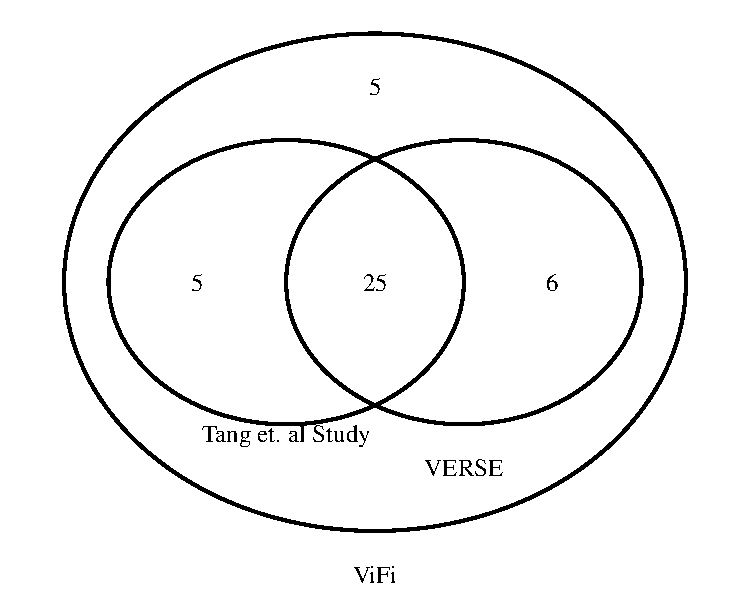
\includegraphics[width=1\linewidth]{results/tcga_triple.pdf}\\
\caption[Venn diagram of fusion reads recovered from the RNA-seq data from Larsson 2013 study]
{\label{venn_diagram}  {\bf Venn diagram of fusion read integration points recovered from the TCGA-CESC samples with matched RNA-seq and WGS sequencing.}  We show a Venn diagram of the overlap of the WGS integration points with a matching mRNA event within 100kb reported by ViFi, VERSE, and the Tang et al. 2013 study on the TCGA-CESC samples with both RNA-seq and WGS sequencing matched pair data.  }
\end{figure}

\paragraph{\textbf{Genome-wide analysis of genomic integrations and fusion mRNA sequences in cervical cancer samples.}}
Having established the concordance of fusion mRNA and genomic
integrations on 28 TCGA-CESC samples explored in the Tang et
al. study, we investigated if these results could be extended to all
68 TCGA-CESC samples with matched WGS and RNA data, and if the
combined analysis could provide new insights into the pathogenicity of
HPV in cervical cancer.

We detected genomic integration in 51 samples of 68 samples (226
integrations total). From RNA-seq data, we detected a total of 376
fusion (viral-human) mRNA junctions, 88\% of which were within 100kbp
of a genomic integration (Fig.~\ref{distance_breakpoint})\footnote{Should we mention
that the remaining 12\% of fusion reads are probably false positives?}; 92\% of
these were within 50kbp, and 70\% within 10kbp. On the other side, 119 (52\%) of
the genomic integrations had at least one
proximal fusion mRNA sequence. Previous studies have shown extensive
alternative splicing in HPV transcripts and HPV fusion
transcripts~\cite{Ziegert2003,Johansson2013}, which explains the
distance from the genomic integration point. These results confirm the
robustness of automated ViFi analysis as well as the strong
concordance between genomic and RNA-seq data.

\begin{figure}[htpb]
  \centering
  \includegraphics[width=1\linewidth]{results/{wgs.rna.histogram.distances}.pdf}\\
\caption[Distance of fusion mRNA breakpoint to nearest WGS integration
  breakpoint.]  {\label{distance_breakpoint} {\bf Histogram of
    distance of fusion mRNA breakpoint to nearest WGS integration
    breakpoint.}  }
\end{figure}


To better understand the pathogenesis of HPV integrations, we first
looked at the annotations near integration points. 67\% of the
integrations had an annotated gene within 10kb of the genomic
integration. Empirical testing of gene counts at random intervals
suggests a modest but significant enrichment of genes near integration
points~(Z-test; p-value $<$ 0.004; Fig.~\ref{integration_counts}).
This result is in concordance with a study by Akagi et al. (2014) on
HPV integration. Next, we examined whether there were recurrent
integrations (integrations from two or more samples within 50kb of
each other) in our dataset and found two genomic regions containing
recurrent integrations: chr13:73955151-74005092 (two samples), and
chr8:128747810-128889296 (four samples).  The first region contains no
nearby genes, and the latter region is within 1Mb of the oncogenes MYC
and PVT1. Both oncogenes have been implicated in recurrent
integrations~\cite{Hu2015}. Third, Hu et al. (2015) also report an
enrichment of genomic instability-related elements near integration
points, including short tandem repeats (STR), short interspersed
nuclear element (SINE-Alu), long terminal repeat/endogenous
retroviruses (LTR/ERV1), fragile X breakpoint cluster repeats, and
satellite DNA. However, these elements are ubiquitous in the genome,
and we did not find any enrichment of similar elements proximal to the
integration sites in our dataset (Methods)\footnote{NOTE: I am
  currently re-running this right now, but I suspect this will hold,
  but will update this statement once it's done.  Elements are short
  tandem repeats (STR), short interspersed nuclear element (SINE-Alu),
  long terminal repeat/endogenous retroviruses (LTR/ERV1), fragile X
  breakpoint cluster repeats, and Satellite}.  Finally, while we did
find a slight enrichment of oncogenes compared to randomly selected
intervals, this finding was not significant. Summarizing, the vast
majority of integrations were not recurrent, nor were they in
oncogenes, and we cannot assert that the location of HPV genomic
integration plays a significant role in CESC pathogenicity. Therefore,
we decided to look at transcript expression near integration.

For each integration, we examined the total transcriptional activity
of the region within 10kb of the sample containing the integration by
comparing region's normalized transcriptional activity as the
transcriptional activity of the same region in all other samples
without the genomic integration.  We find a significant increase in
expression (\VB{P-value}) ($2.83\times$ average) across all genomic
segments with integrations (Fig.~\ref{all_expression}).  Remarkably,
the increased expression is highly correlated with the presence of a
fusion transcript (Fig.~\ref{expression_transcripts}).  There is a
$7.41\times$ average increase if the genomic segment contains a fusion
mRNA sequence, versus a small decrease ($0.97\times$) when no fusion
mRNA is seen.


\begin{figure}[htpb]
  \centering
  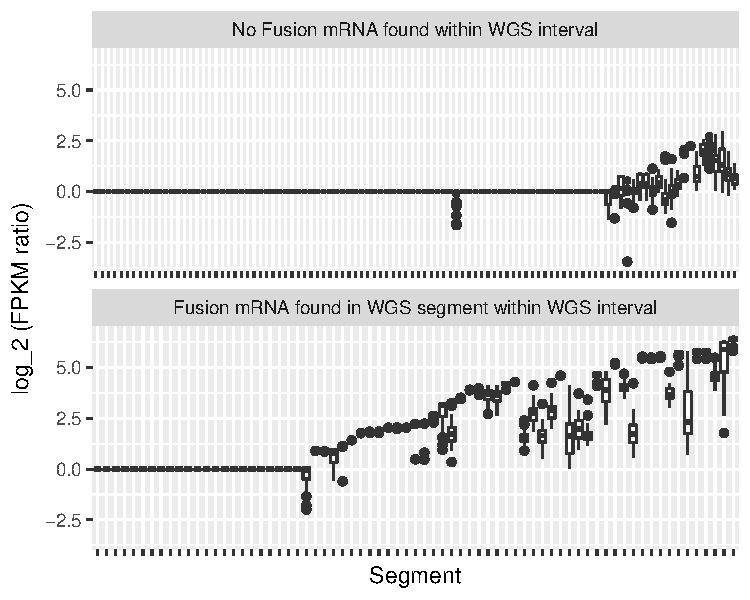
\includegraphics[ width=1\linewidth]{{results/wgs.fpkm.fusion.boxplot.10000}.pdf}\\
\caption[Log$_2$-fold change of expression between genomic segments with
  and without integrations.]  {\label{all_expression} {\bf Boxplots of
    log-fold change of expression between genomic segments with and
    without integrations.}  We show boxplots of the Log$_2$-fold change
  in expression of genomic regions with and without integrations.  The
  genomic regions are separated by whether or not there are associated
  fusion transcriptions within the interval containing the genomic integration.}
\end{figure}

The observation that integration is correlated with increased
expression leaves us with two important questions.  First, how does
the increased expression contribute to pathogenesis.  Second, what
causes the increase in expression, and in particular, why is this
increase more prominent when fusion mRNA sequences are observed.



%In order to determine what these transcripts are and what role they
%might play in pathogenicity, we started by annotating the expressed
%transcripts proximal to genomic integrations.  For each genomic
%segment containing an integration, we took all positions within 10kb
%interval of the integration that were covered by at least three or
%more mRNA reads, and then clustered the positions into intervals.  We
%merged any intervals that were within 5 bps of another interval.
% We also computed the expected number of annotations observed from randomly selected
%segments as a baseline for comparison.  We found that regions with
%integrations were not only statistically significantly enriched in
%transcript annotations for genes~(Z-test; p-value $<$ 1e-20;
%Fig.~\ref{transcript_count})), but also for repeat elements such as
%DNA repeat elements, SINEs, LINEs, and LTRs~(Z-test; p-value $<$
%1e-20; Fig.~\ref{transcript_count}; see
%Fig.~\ref{transcript_count_all} for all other repeat elements).
%Specifically, we see a two-fold increase in the total number of gene
%annotations of transcripts. Even more interesting, we see more than a
%12-fold increase in LINE and LTR annotations of transcripts. 


To answer the first question, we observed that 39\% of the
integrations had no gene within a 10kb interval, but we still observed
transcripts from 49\% of those regions. To understand the function of
the transcripts, we marked all transcribed genomic intervals (Methods)
and compared against RefSeq genes~\cite{OLeary2016} or
RepeatMasker~\cite{Tarailo-Graovac2009} annotations. For each
integration and a class of annotations (e.g. LINE), we counted the
fraction of annotated elements that were transcribed, and compared
that with the fraction of annotated elements of the same class in
randomly selected segments (Fig.~\ref{transcript_count}). We found
that genes (p-val$:XXX$), LINEs (p-val$:XXX$), SINEs (p-val$:XXX$),
LTRs (p-val$:XXX$) were all much more likely to be transcribed in the
proximity of an integration site. Genes were twice as likely, and
LINEs and LTRs were $12\times$ more likely to be transcribed. Recall
that we had seen no statistically significant difference between the
number of LINE and LTR annotations at the genomic level. While repeat
elements are ubiquitous throughout the genome, they are much more
likely to be transcribed in the proximity of a viral integration
(Fig.~\ref{expression_transcripts}).

%transcribed regions near integrations
%refer to methods, clear explanation of statistical test
%talk about which tested and enrichment of what
%Noteably in xxx regions no genes in the region, but lines/ltrs expressed

This surprising result suggests one potential avenue for increased
pathogenicity: genomic instability and pathway disruption caused by
expression of LINE and LTR elements that are normally silent. L1
elements are retrotransposons and have been shown to create double
stranded breaks in the host cell genome when transcribed, leading to
genomic instability~\cite{Gasior2006}.  Similarly, LTRs can act as
promoters, enhancers, and transcriptional factor-binding sites, and
can potentially be transcriptionally active, depending on the
tissue~\cite{Yu2013}. LINEs and LTRs are both epigenetically repressed
in somatic cells~\cite{Kinomoto2007,Sigurdsson2012}, but have been
shown to be active in selected
neoplasms~\cite{Rodic2013,Xiao-Jie2016,Romanish2010}. We found a four
to five-fold increase in transcription expression of these elements in
regions proximal to integration sites (p-val:$xxx$,
Fig.~\ref{expression_transcripts}).

\begin{figure}[htpb]
  \centering
  \includegraphics[width=1\linewidth]{results/{expected.rna.counts.violin}.pdf}\\
\caption[Annotations of transcripts covering the regions containing integrations.]
{\label{transcript_count}  {\bf Observed and expected annotation counts of transcripts covering the genomic segment containing integrations.}  We show the violin plots of the expected number of annotations of transcripts from random intervals over 1000 replicates, and the actual number of annotations of transcripts for the observed integrations found in our TCGA-CESC dataset (in red).  The quantiles of the violin plots are displayed with lines.  The p-values of the observed annotation counts (Z-test) are all statistically significant (p-value < 1e-20).}
\end{figure}

To understand why genomic integration and fusion transcripts are
correlated with increased transcription, we started by characterizing
the orientation of fusion transcripts. As the RNA-sequencing library
preparation was not strand specific, we could not determine the active
strand directly. However, because HPV genes are known to be
transcriptionally active in cervical cancer
cells~\cite{Johansson2013}, we can assume that the majority of viral
transcripts should be oriented in the same direction as the viral
gene.  Using this assumption, we could determine if the human portion
of a fusion transcript was upstream or downstream of the viral
gene. 82\% of fusion mRNA sequences showed the human fragment to be
downstream of the viral genes.  (Fig.~\ref{mrna_directions}). Of the
remaining 18\% of the sequences where the human portion was upstream
of the viral gene, 87\% were within 10kb of an annotated gene.  These
observations suggest that transcription of fusion mRNA sequences are
largely driven by the upstream regulatory elements within the viral
genome.  In the rare cases in which the viral gene is downstream of
the human portion of the fusion transcript, human regulatory elements
may drive expression.

%, but a fold change of 0.86 to 0.92 when no fusion mRNA is presents

To better characterize how the integration might drive downstream
expression, we performed a more detailed analysis of the
transcriptional activity local to the integration site.  For each
genomic integration, we categorized the integration as a simple,
complex, or fusionless integration site (Fig.~\ref{updown}a).  We
define simple integrations as a single integration within the 10kb
interval with the chimeric paired-end reads being concordant, allowing
us to identify regions upstream and downstream of the viral gene. In
contrast, define complex integrations as regions containing multiple
fusion mRNA sequences with discordant chimeric paired reads. Finally,
regions without chimeric RNA are denoted as `fusionless'. Using these
definitions, we characterized 68, 51, and 107 integrations as simple,
complex, and fusionless, respectively.

%as either having two or more integrations within the 10kb interval
%that are sufficiently far apart that we can detect them as being
%separate integrations, or a cluster of integrations that is detected
%as a single integration event.  This cluster can produce

We observed (as before) that in the presence of fusion mRNA (simple or
complex), there is a two- to five-fold increase in expression
(p-val:$xxx$) local to the integration point (Fig.~\ref{updown}b).
The increase in expression can be evident up to 100kb around the
integration point (Fig.~\ref{updown_250kb}).  In the case of simple
integrations, there is a clear increase downstream of the integrated
viral sequence.  Finally, fusionless integrations show a slight
decrease in expression.

Taken together, our results are consistent with the following model:
HPV integrates into a random location and causes dysregulated
expression of all proximal elements possibly driven by the viral
regulatory elements. This can result in transcription of elements that
are normally silent or not expressed in normal samples. When the
insertion is proximal to LINE/LTR elements, there is an increase in
genomic instability.

\begin{figure}[htpb]
  \centering
  \subfloat[Classification of integration points.]{\includegraphics[width=4in,frame]{{classification}.pdf}}\\
  \subfloat[Log$_2$fold expression near integration point.]{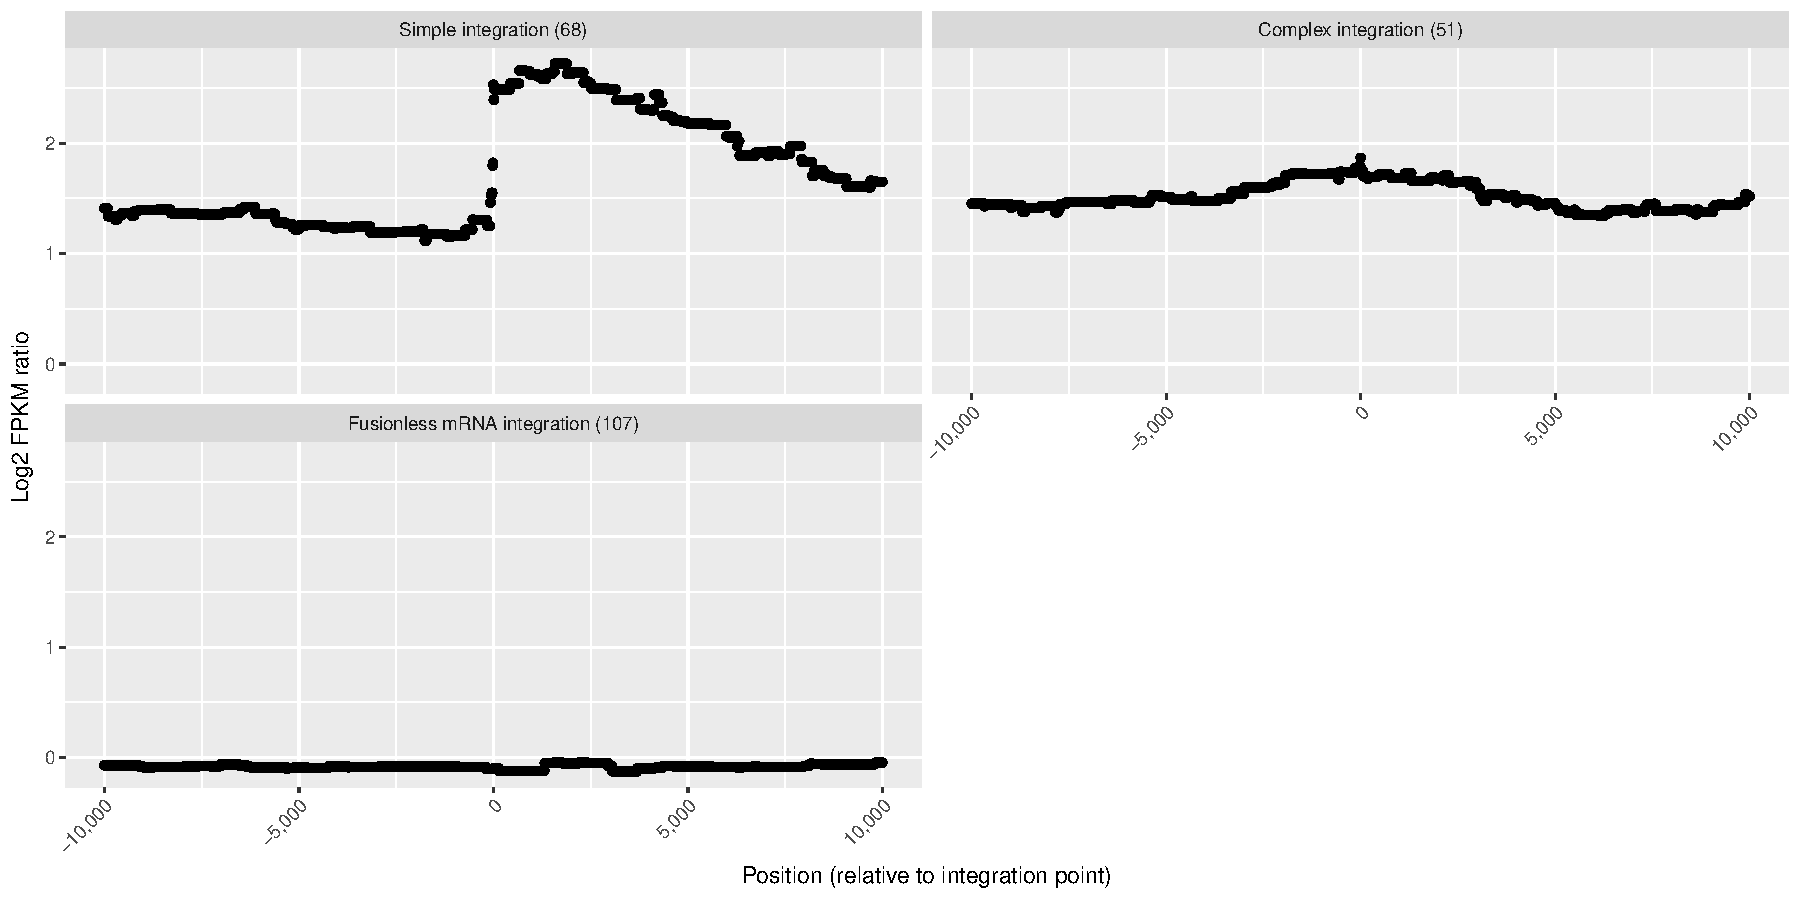
\includegraphics[width= 4in,frame]{{results/updown.10000}.pdf}}
\caption[Fusion reads supp.]
        {\label{updown}  {\bf Categorization of integration points and expression change around integration point}.  a) We categorize integration points into three categories: simple integration, complex integration, and fusionless mRNA integration.  Simple integrations have no other integrations within a 10kb window, and at least 75\% of the chimeric paired-end reads supporting a fusion mRNA event are oriented in the same direction.  Complex integrations either have multiple integration events within a 10kb window, have multiple fusion mRNA supporting different orientations, or have chimeric paired-end reads that support conflicting orientations for the same mRNA fusion event.  Integrations that have no fusion mRNA events are categorized in a separate category.  b) We report the average log-fold expression change upstream and downstream of an integration event.  The position is reported relative to the integration point in the human genome, with negative position being upstream of the integration event, and positive position being downstream of the integration event.  The results are separated out by the integration category.  In total, there are 68 simple integrations, 51 complex integrations, and 107 integration events with no fusion mRNA sequences.} %35,
\end{figure}

\section*{Discussion}
We present ViFi, a new method for detection of viral integration sites
and fusion mRNA sequences.  The key advances of ViFi are the use of
eHMMs to better detect evolutionarily divergent viruses and the use of
mappability scores to reduce false positive detections.  Our
simulation experiments shows that ViFi has high precision and
sensitivity in detecting viruses, even under difficult conditions of
highly mutated or novel viral strains.  VERSE, on the other hand,
performs poorly or fails to detect integration on the hardest model
conditions.  On the biological datasets, ViFi detects more integration
events than VERSE.  ViFi is computationally efficient and its running
time is not dramatically impacted the number of viral integrations,
whereas VERSE is unable to complete analyses within 48 hours on
datasets with 1,000 integrations.

Previous research on the role of viral integration on tumorigenesis
focused on identifying genomic hotspots containing recurrent
integrations and identifying change in both host and viral gene
expression resulting from
integration~\cite{Sung2012,Tang2013,Lawrence2015,Hu2015,Zhang2016}.  Previous
observations showed that recurrent integrations often occurred near
known oncogenes such as MYC, PVT1, ERBB2, RAD51~\cite{Tang2013}, but
our results show that recurrent integrations are very rare.  Hu et
al. (2015) suggested that HPV integrates randomly across the genome
until an integration occurs in a region that provides a proliferative
advantage, resulting in oncogenesis.  However, the vast majority of
integrations are non-recurrent and the majority of samples do not have
integrations in or near oncogenes.  Thus, focusing on genes with
recurrent integrations can only explain samples that have integrations
in those genes, potentially ignoring a large portion of samples that
do not contain integrations in recurrent regions.

Our results show that viral integration plays a powerful role on local
transcriptional activity, especially when fusion human-viral mRNA
sequences are present.  This includes a strong increase in
transcription near the integration site, as well as transcription of
elements that might normally not be expressed.  Our results are
consistent with the theory that integration results in the recruitment
of transcription factors by HPV's upstream regulatory region (URR) and
subsequent transcription read-through to produce both viral-human mRNA
transcripts as well as an uptick of expression downstream from the
viral integration point.  More interestingly, our results also suggest
that this increase in expression might also be due to human-viral
ecDNA structures that are unbound to the chromatin.  ecDNA structures
can be independently amplified as well as allow for unregulated
transcription; these two facts might explain the wide variation we see
in transcription levels for the different integration points.  Further
research is necessary to see if we can experimentally verify the
existence of human-viral ecDNA structures.

The production of fusion transcripts may also play a role in tumor
progression.  Viral-human fusion transcripts can alter functional
pathways, as in the case of the viral-human fusion transcript
HBx-LINE1~\cite{Lau2014,Liang2016}, which acts as a sponge for
miRNA-122 and promotes hepatic cell epithelial-mesenchymal transition
(EMT)-like changes and increases susceptibility to induced tumor
formation~\cite{Liang2016}.  Recent studies for HPV-related cancers
have noted differential expression profiles of miRNAs for HPV-positive
and HPV-negative samples~\cite{Lajer2012,Gao2016}.  One possibility is
that fusion transcripts produced by integrated HPV might also act as a
sponge for miRNA.  Another possibility is that fusion transcripts
might better disrupt host cellular pathways.  Jeon and Lambert (1995)
found that viral mRNA from integrated HPV are more stable due to the
resulting disruption of the mRNA instability element in the viral
genome after integration~\cite{Jeon1995}.  Thus, fusion mRNA might
also be more stable, especially in light of the observation that the
human portion is typically downstream of the viral portion in fusion
mRNA sequences.


The question about why viral integration leads to dysregulation of
expression is not fully resolved. Recent studies have shown the
presence of extrachromosomal circular (ecDNA) in nearly half of all
cancers, with amplified driver oncogenes were commonly found on
ecDNA~\cite{Turner2017}. Oncogenes on ecDNA show higher expression
presumably because they are more accessible. We found through a close
inspection of several integrations that the segments from the human
and viral genomes could be arranged in a cyclic structure
(Fig.~\ref{tcga_c5_a0tn}).  For example, the sample TCGA-C5-A0TN had
235 chimeric paired-end reads between chr2:195586245 and HPV16:2593,
149 discordant paired-end reads between chr2:195603512 and
chr3:126826267, and 229 chimeric paired-end reads between
chr3:126849186 and HPV:6071 (Fig.~\ref{tcga_c5_a0tn}a). It is not
implausible that human-viral ecDNA might also exist, especially
because HPV can exist in both integrated and episomal forms within
cervical cells~\cite{Williams2011,Shin2014}, and that would explain
both local copy number amplification near integrated
regions~\cite{Akagi2014} as well as higher expression in the proximal
region. This is an exciting hypothesis that warrants further
investigation.

\begin{figure}[htpb]
  \centering
  \subfloat[TCGA-C5-A0TN.]{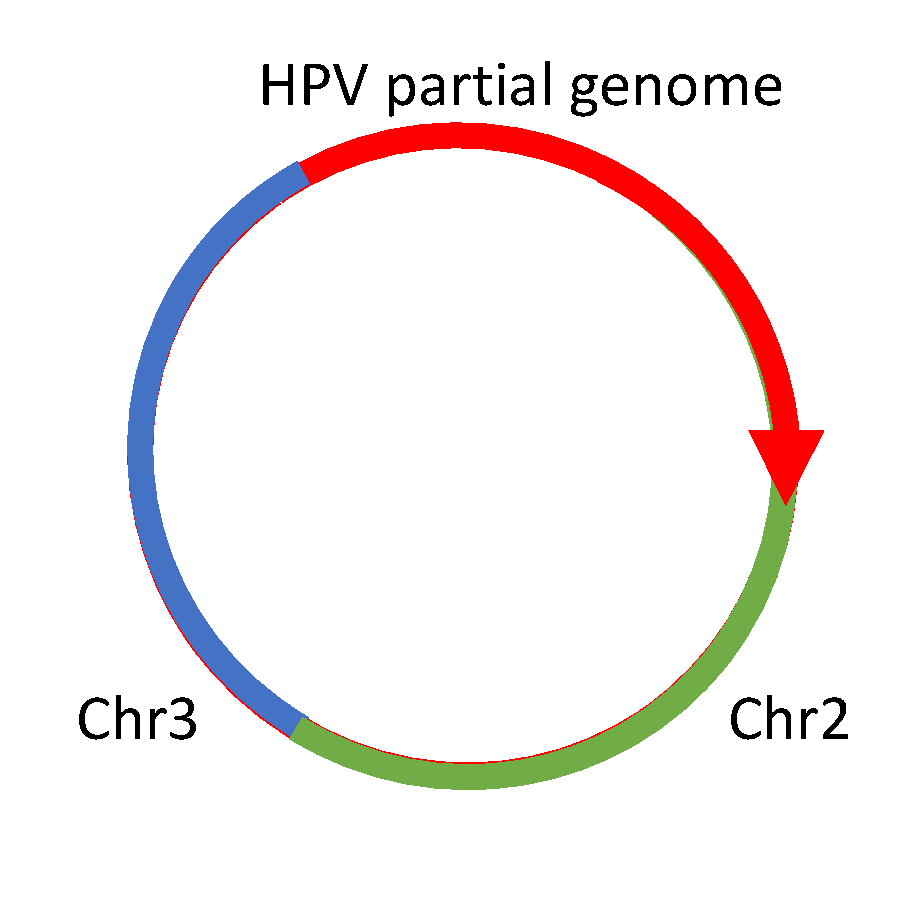
\includegraphics[width=3in,frame]{{results/episome}.pdf}}
  \subfloat[TCGA-EK-A2RE.]{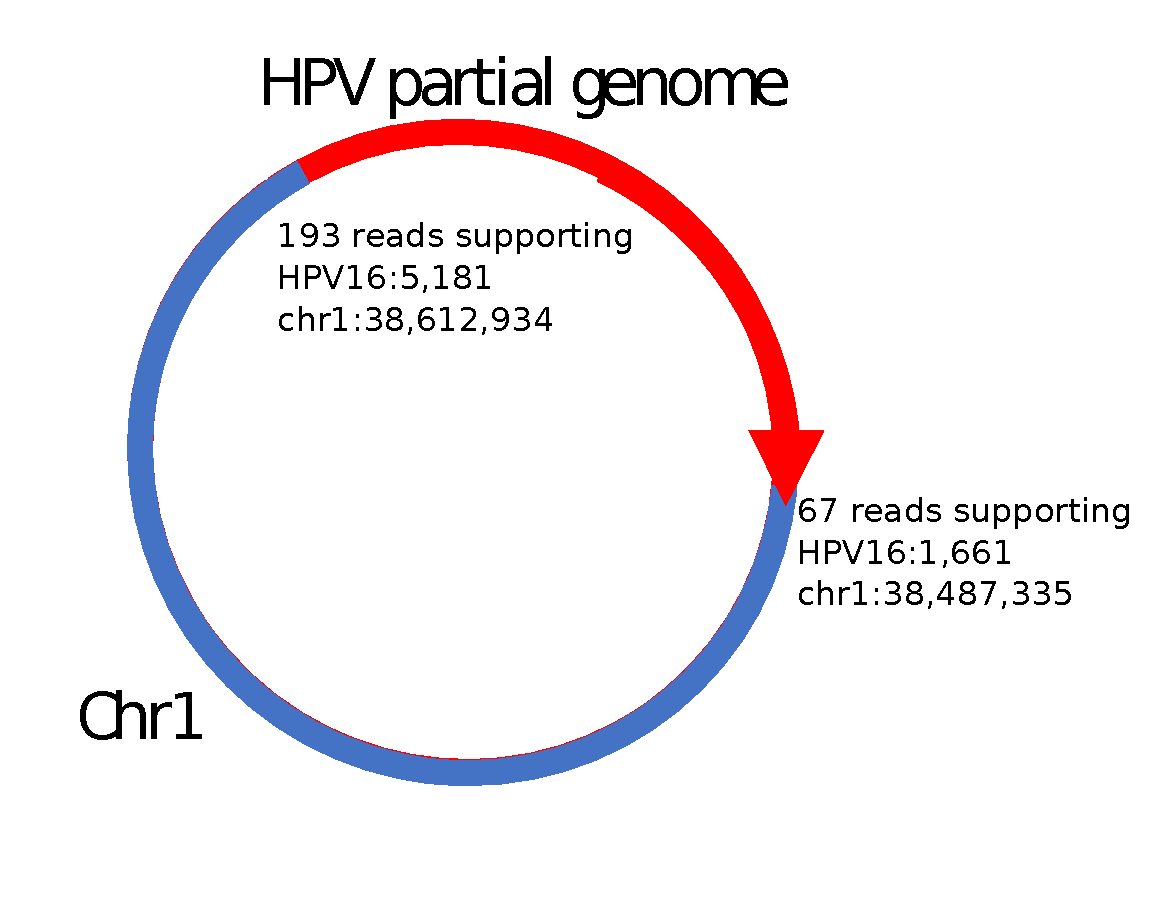
\includegraphics[width=3in,frame]{{results/episome-TCGA-EK-A2RE}.pdf}}\\  
\caption[Examples of hypothetical ecDNA structures.]
{\label{tcga_c5_a0tn}  {\bf Examples of hypothetical ecDNA structures.}  a) Hypothetical ecDNA structure for an integration from TCGA-C5-A0TN and b) hypothetical ecDNA structure for an integration from TCGA-EK-A2RE.  The number of paired-end reads supporting each boundary is shown.}
\end{figure}




%One possible direction to better understand the role of LINE and LTR expression is combining proteomics and genomics.  In particular, focusing on whether HPV positive samples with integration show higher expression of L1 encoded proteins, ORF1p and ORF2p, compared to HPV positive samples without integration.  
 
\section*{Method}
\paragraph{\textbf{ViFi.}}
We present \textbf{V}irus \textbf{I}ntegration and \textbf{F}usion \textbf{I}dentification (ViFi), a new pipeline for detection of integration sites (Fig.~\ref{flowchart}).  Unlike other integration detection pipelines that use reference-based alignment mapping for identifying viral reads, ViFi uses a combination of reference-based alignment mapping and ensemble of profile HMMs to identify viral reads.  

\paragraph{\emph{Pre-processing.}} ViFi begins with a pre-processing step (see Fig.~\ref{flowchart}a) that builds a BWA index for the human reference genome and viral genomes (Hg19+viral index).  In addition, ViFi takes the genomes from the viral family and estimates a MSA on each family using PASTA~\cite{Mirarab2014}.  A maximum likelihood (ML) tree is estimated from the alignment using RAxML~\cite{Stamatakis2014}.  Next, ViFi builds an ensemble of HMMs from the alignment and tree using HIPPI~\cite{Nguyen2016_hippi}.  Briefly, a profile HMM is computed on the input MSA and ML tree.  Next, the ML tree is partitioned into two subtrees by taking its centroid edge (i.e., the edge that best separates the tree into two subtrees with roughly equal number of leaves).  Profile HMMs are then built on the alignments induced by the leaf set of each of the subtrees.  The process repeats recursively on each subtree until there are at most 10 sequences in the subtree.  This results in a collection of nested hierarchical profile HMMs which we call the ensemble of HMMs.  This pre-processing step of building the ensemble of HMMs only needs to be run once for each viral family of interest.

\paragraph{\emph{Identification of candidate reads.}} Similar to other existing viral integration detection pipelines, the first step of ViFi is to align each paired-end read to the Hg19+viral index (see Fig.~\ref{flowchart}b).  The paired-end reads are separated into four different groups: i) reads in which both paired-end reads mapped Hg19 or both to the viral genomes, ii) paired-end reads in which one end mapped to Hg19 and the other to a viral genome, iii) paired-end reads in which one end mapped to Hg19 and the other is unmapped, and iv) all other reads.  Typically, most existing viral integration detection pipelines focus on the set of reads in group ii) and discard reads found in group iii).  However, a read that is viral in origin might be unmapped because it is too evolutionarily divergent from the set of known viral genomes.  Our method attempts to rescue paired-end reads in this category by scoring the unmapped reads against the ensemble of HMMs created in the pre-processing step.  If a read has a sufficient score to one of the HMMs in the ensemble (E-value of 0.01 or lower), then the read is marked as a viral read and the paired-end read is put into the candidate set, along with all reads from group ii).  This step allows the detection of novel or evolutionarily divergent viral sequences belonging to the same family.  The last step is to infer integration from the set of candidate reads.  

\paragraph{\emph{Identification of integration point.}}  The set of candidate reads are ordered by coordinates of the human genomic position.  Read pairs with poor mappability scores, defined as Duke Uniqueness Score~\cite{unknown} less than 0.33 or MAPQ score less than 10 are removed.  These removed reads represent reads that might map to multiple locations.  The remaining read pairs within 300 bps of each other are clustered into a group of read pairs supporting the integration point.  The reads remaining in the cluster are then considered highly supported reads (i.e., have high mapping score).  

%Any paired end reads in which one or more ends did not map to the reference are put into a candidate set.  From the candidate set, all reads are scored against the ensemble of HMMs, and those that score above a threshold are marked as viral.  paired end reads that have at least one read mapping to the human reference and one marked viral are considered candidate integration points.  Integration points with at least three paired end reads supporting the integration are listed as positive integrations.


%paired end reads in which at least one end did not map to the human reference are put into a candidate set.  All reads in the candidate set are scored against each HMM in the ensemble using nhmmer from the HMMER suite of tools~\cite{Eddy1998}.  Any read that scores above a threshold $T$ is marked as viral.  paired end reads in which at least one end maps to the human reference and at least one end is marked as viral are considered as candidate integration event.  Any read that maps to the human reference and is marked as viral is candidate split read and is used to identify the integration point on the human genome.  If an integration point is covered by a split read, we can identify the exact integration location on the human genome.  However, as not all integration events are covered by split reads, we also identity integration points with a range (ADD MORE DETAIL) defined by the insert size.  Integration points that are supported by three or more paired end reads are outputted as  true integration points.

\begin{figure*}[htpb]
  \centering
  \subfloat[Pre-processing]{\includegraphics[width=4in,frame]{{preprocess}.pdf}}\\
  \subfloat[Pipeline]{\includegraphics[width= 4in,frame]{{mapping}.pdf}}
\caption[Overview of integration detection pipeline.]
{\label{flowchart}  {\bf Overview of integration detection pipeline.}  Integration detection is split into two phases.  In the a) pre-processing step, a BWA index is created from the human reference genome and input viral genomes (Hg19+viral).  In addition, a multiple sequence alignment (MSA) is estimated from the viral genomes, and an maximum likelihood (ML) tree is estimated from the alignment.  The MSA is decomposed into an ensemble of profile Hidden Markov models.  In the b) viral detection step, the paired-end reads are mapped against the Hg19+viral index.  Candidate paired-end reads are selected if, i) one end of the read maps to the human genome and the other end maps to a viral genome, or ii) one end of the read maps to the human genome and the other end scores high against the HMM ensemble.  All other reads are discarded.  The integration point is then inferred from the set of candidate reads.
% i) reads in which both paired end reads mapped Hg19 or both to the viral genomes, ii) paired end reads in which one end mapped to Hg19 and the other to the viral genomes, iii) 
%Any paired end reads in which one or more ends did not map to the reference are put into a candidate set.  From the candidate set, all reads are scored against the ensemble of HMMs, and those that score above a threshold are marked as viral.  paired end reads that have at least one read mapping to the human reference and one marked viral are considered candidate integration points.  Integration points with at least three paired end reads supporting the integration are listed as positive integrations.
}
\end{figure*}


\begin{figure}[htpb]
  \centering
  \includegraphics[width=0.6\linewidth]{{ehmm}.pdf}\\
\caption[Ensemble of HMMs technique.]
{\label{ehmm}  {\bf Algorithm for generating the ensemble of HMMs.}  The input is a initial MSA and a maximum likelihood (ML) tree that has been estimated for the MSA. The algorithm begins by adding the HMM built on the MSA to the ensemble. If the MSA has more than 10 sequences, the ML tree is decomposed into two subtrees by deleting the centroid edge (i.e., the edge that produces a maximally balanced split of the sequence set into two sets). The subtrees are used to generate induced alignments. HMMs are built for each induced alignment and added to the ensemble. The process iterates on those subtrees that meet the criterion for decomposition (subset size more than max(10, n/10), where n is the number of sequences in the initial MSA, and mean pairwise sequence identity less than 0.4).}
\end{figure}

\paragraph{\textbf{Datasets.}}  We use both simulated and biological datasets in our studies.  We describe the datasets below.

\paragraph{\emph{HPV simulated WGS datasets (HPV-Sim)}}
We simulated 16 human genomes with HPV integrations.  In order to examine the impact of viral sequence divergence on integration detection, we simulated different strains of HPV by evolving HPV16 down a phylogenetic tree with differing branch lengths.  We grouped the simulations into three categories, depending on the integrating virus strain's similarity to the reference HPV16 strain: easy (99\% similarity), medium (95\% similarity), and hard (90\% similarity).  In addition, we generated one additional dataset with Brown Howler PV (AgPV1), a papillomavirus genome not included in the set of viral reference genomes to simulate detection of a novel HPV virus.  AgPV1 is 44\% similar to HPV16 and is 65\% similar to the most closely related sequence in the set of reference genomes.


\paragraph{\emph{HCC Sung 2012 WGS dataset (HCC-WGS)}}
88 HCC samples (81 HBV-positive and 7 HBV-negative; both tumor and adjacent tissue) were sequenced by Sung et al.~\cite{Sung2012}.  The authors identified recurrent breakpoints (4 or more samples) in known oncogenes/oncogenic regions (FN1, TERT, MLL4, CCNE1, ROCK1, SENP5).  A total of 399 breakpoints were identified across the 88 samples.  To confirm recurrent breakpoints, the authors randomly selected 32 breakpoints in six affected genes from 21 samples and validated 22 of these (72\%) via PCR.  Our study used the same 21 samples in our comparison.

\paragraph{\emph{HCC Lau 2014 cell line RNA-seq dataset (HCC-RNAseq)}}
Whole transcriptomes from four HCC cell lines were analyzed using RNA-seq~\cite{Lau2014}.  11 chimeric HBV-human fusion transcripts in three of the cell lines were detected and validated using Sanger sequencing.  Our study included the original six cell line RNA-seq data.  

\paragraph{\emph{TCGA Cervical cancer datasets (TCGA-CESC)}}
We found 68 patient cervical tumor samples in the TCGA database~(\url{https://cancergenome.nih.gov/}) with matched WGS and RNA-seq tumor sequencing data.  Of the 68 samples, 28 samples overlapped with the Tang et al. study~\cite{Tang2013} which examined the landscape of mRNA viral fusion events across the TCGA dataset.  Our study includes a comparison of ViFi and VERSE to the results of the Tang study on the 28 samples, as well as analyses on all 68 samples.


\begin{table*}[htb]
\centering
\caption{\textbf{Overview of datasets}.  We provide an overview of the datasets used throughout this study.  }
\label{table:data}
\begin{tabular}{|l|l|l|r|r|}
\hline
Dataset name & Type & Source & Number of samples & Source \\ \hline
HPV-Sim & WGS &Simulated& 16 & Generated for this study \\ \hline
HCC-WGS & WGS & Biological&20 & ~\cite{Sung2012} \\ \hline
HCC-RNA & RNA-seq & Biological&6 & ~\cite{Lau2014} \\ \hline
TCGA-CESC & WGS and RNA-seq &Biological& 68 & TCGA~\cite{TODO} \\ \hline 
\end{tabular}
\end{table*}

%\subsection{HCC WGS patient results}
%Of the 22 experimentally verified integration points, Viral-HMM was able to detect 21 of the points, VERSE 8 of the points, and ...  Note that in the VERSE paper, the authors reported that they were able to detect 16 out of the 22 points.  We had difficulties in running VERSE on our samples, and tools used within the VERSE pipeline produced very large uncompressed SAM files (up to 1.2 TB in size).  We attempted to fix this by having VERSE output compressed BAM files, which allowed several of the failed runs to complete, but not all.  We suspect that with more efficient use of piping, VERSE could avoid producing many of the large files and would be able to complete on our system and potentially achieve the results reported in their paper.

%\begin{table*}[]
%\centering
%\caption{HCC WGS patient results.  Results on detection of 22 experimentally verified integration points across 13 samples taken from patients with HCC.}
%\label{my-label}
%\begin{tabular}{|l|l|l|l|l|l|}
%\hline
%Sample & Integration breakpoints in human genome & Viral-HMM & Viraj & VERSE                                & VirusSeqFus \\\hline
%145T   & chr19: 30303492                         & Y         &       & Y                                    & Running     \\\hline
%       & chr19: 30303498                         & Y         &       & Y                                    & Running     \\\hline
%177T   & chr3: 196625752                         & Y         &       & N                                    & Running     \\\hline
%180N   & chr2: 216280279                         & Y         &       & Running & Running     \\\hline
%186T   & chr19: 36214005                         & Y         &       & Y & Running     \\\hline
%       & chr19: 36214017                         & Y         &       & Y & Running     \\\hline
%198T   & chr5: 1269387                           & Y         &       & Y                                    & Running     \\\hline
%       & chr5: 1269405                           & Y         &       & Y                                    & Running     \\\hline
%26T    & chr18: 107920                           & Y         &       & Running & Running     \\\hline
%200T   & chr19: 30315003                         & Y         &       & Y & Running     \\\hline
%       & chr19: 30315365                         & Y         &       & Y & Running     \\\hline
%268T   & chr19: 30298787                         & Y         &       & Y                                    & Running     \\\hline
%       & chr5: 1292391                           & Y         &       & N                                    & Running     \\\hline
%43T    & chr3: 196625710                         & Y         &       & N                                    & Running     \\\hline
%46T    & chr5: 1295367                           & Y         &       & N                                    & Running     \\\hline
%70T    & chr19: 36212331                         & Y         &       & Running & Running     \\\hline
%       & chr19: 36212311                         & Y         &       & Running & Running     \\\hline
%71T    & chr3: 196625776                         & Y         &       & N                                    & Running     \\\hline
%       & chr19: 36213141                         & Y         &       & Y                                    & Running     \\\hline
%       & chr19: 36213136                         & Y         &       & Y                                    & Running     \\\hline
%       & chr5: 1292403                           & N         &       & N                                    & Running     \\\hline
%95T    & chr19: 36212564                         & Y         &       & Y                                    & Running    \\\hline
%\end{tabular}
%\end{table*}
\section*{Data Access}

\section*{Acknowledgements}
The results published here are in whole or part based upon data generated by the TCGA Research Network: \href{http://cancergenome.nih.gov/}.


\section*{Disclosure Declaration}
VB is a partner in Digital Proteomics, LLC (DP), which licenses and sells computational tools for analyzing mass spectrometry data. The terms of this arrangement have been reviewed and approved by the University of California, San Diego in accordance with its conflict of interest policies. DP was not involved in the research presented here

%\bibliographystyle{natbib}
%\bibliographystyle{achemnat}
%\bibliographystyle{plainnat}
%\bibliographystyle{abbrv}
%\bibliographystyle{bioinformatics}
%
%\bibliographystyle{plain}
%
%\bibliography{Document}

\bibliographystyle{genres}
\bibliography{main}

\section*{Online supplemental materials}
\setcounter{figure}{0}
\renewcommand{\thesection}{S.\arabic{section}}   
\renewcommand{\thefigure}{S\arabic{figure}}   
\renewcommand{\thetable}{S\arabic{table}}   

\begin{figure}[htpb]
  \centering
  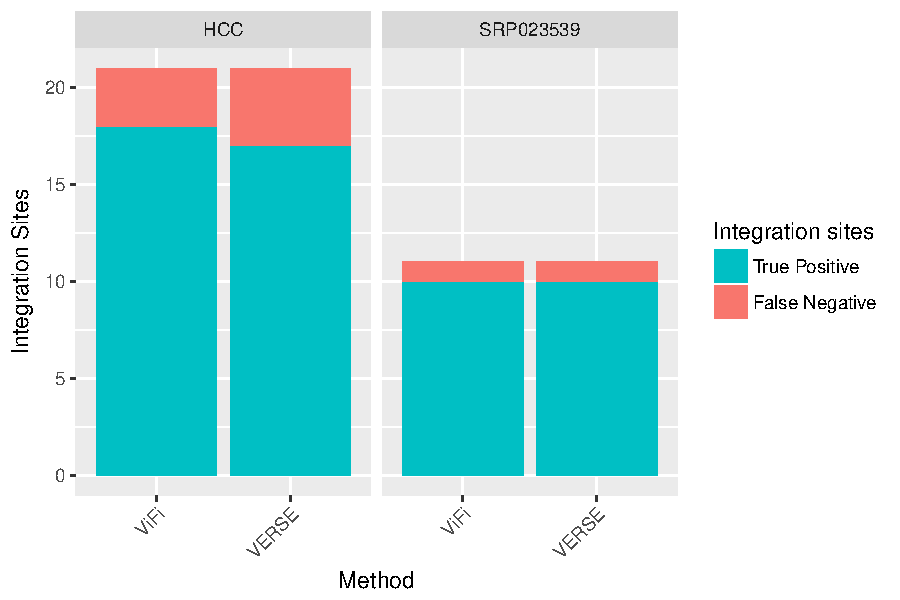
\includegraphics[width=1\linewidth]{results/hcc.pdf}\\
\caption[Recovery of experimentally verified integration sites from biological datasets.]
{\label{bio_results}  {\bf Recovery of experimentally verified integration sites.}  We report the number of experimentally verified integration sites recovered from biological datasets for our method and VERSE.  The datasets include the HCC WGS dataset from the Sung et al. 2012 study (21 experimentally validated integration sites) and the HCC RNAseq cell line dataset from the Lau et al. 2014 study (11 experimentally validated integration sites).}
\end{figure}

\begin{figure}[htpb]
  \centering
  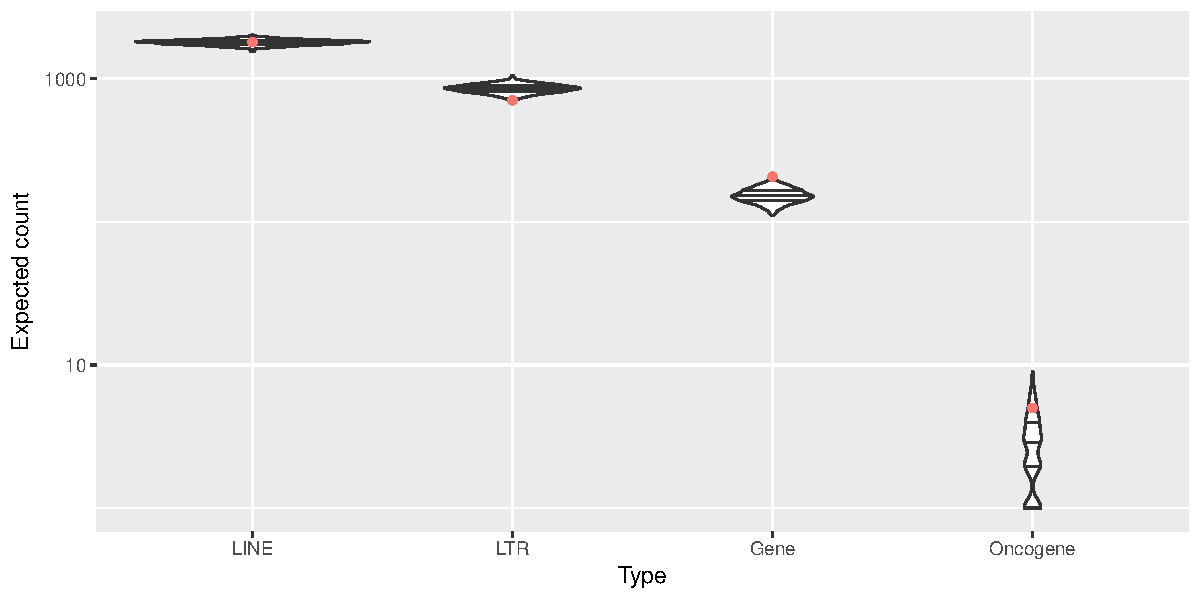
\includegraphics[width=1\linewidth]{{results/expected.counts.violin}.pdf}\\
\caption[Annotations of integrated regions.]
{\label{integration_counts}  {\bf Observed and expected number of annotations of the integrated regions.}  We show the violin plots of the expected number of counts from random integrations for each annotation over 1000 simulated experiments, and the actual number of annotations for the observed integrations found in our TCGA-CESC dataset (in red).  The quantiles of the violin plots are displayed with lines.  The p-values of the observed annotation counts (Z-test) are: LINE $<$ 0.882;	LTR $<$ 0.013;  Gene $<$ 0.004; and	Oncogenes $<$ 0.179.}
\end{figure}

\begin{figure}[htpb]
  \centering
  \includegraphics[width=1\linewidth]{results/{expected.rna.counts.violin.all}.pdf}\\
\caption[Annotations of gene and all repeat elements for transcripts covering the regions containing integrations.]
{\label{transcript_count_all}  {\bf Observed and expected gene and repeat annotation counts of transcripts covering the genomic segment containing integrations.}  We show the violin plots of the expected number of annotations of transcripts from random intervals over 1000 replicates, and the actual number of annotations of transcripts for the observed integrations found in our TCGA-CESC dataset (in red).  The quantiles of the violin plots are displayed with lines.}
\end{figure}


%\begin{figure}[htpb]
%  \centering
%  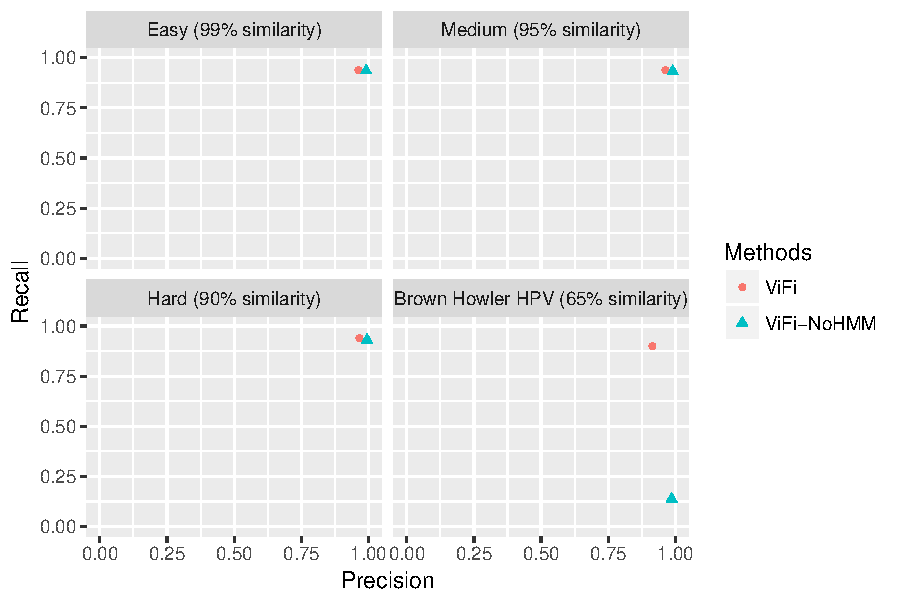
\includegraphics[width=1\linewidth]{{results/simulation.1000}.pdf}\\
%  \caption[Precision-recall on simulated datasets with 1000 viral integrations.] {{\bf Precision-recall on simulated datasets.  \label{sim_results_1000}}  We report the recall and precision for four different model conditions.  We show results for when we include the usage of the  ensemble of HMMs in detecting viral reads (Default) and when we exclude the usage of the ensemble of HMMs (Default-NoHMMs).  The first three model conditions (easy, medium, and hard) vary the percent similarity of simulated HPV16 genomes to the reference HPV16 genome, with five replicates per simulation.  The last model condition uses Alouatta guariba papillomavirus 1 (AgPV1), an HPV genome not included in the set of viral genomes to simulate detection of a novel HPV virus.  AgPV1 is 44\% similar to HPV16.  VERSE failed complete on any datasets.  All datasets were simulated with 25x coverage.}
%\end{figure}

%\begin{figure}[htpb]
% \centering
% 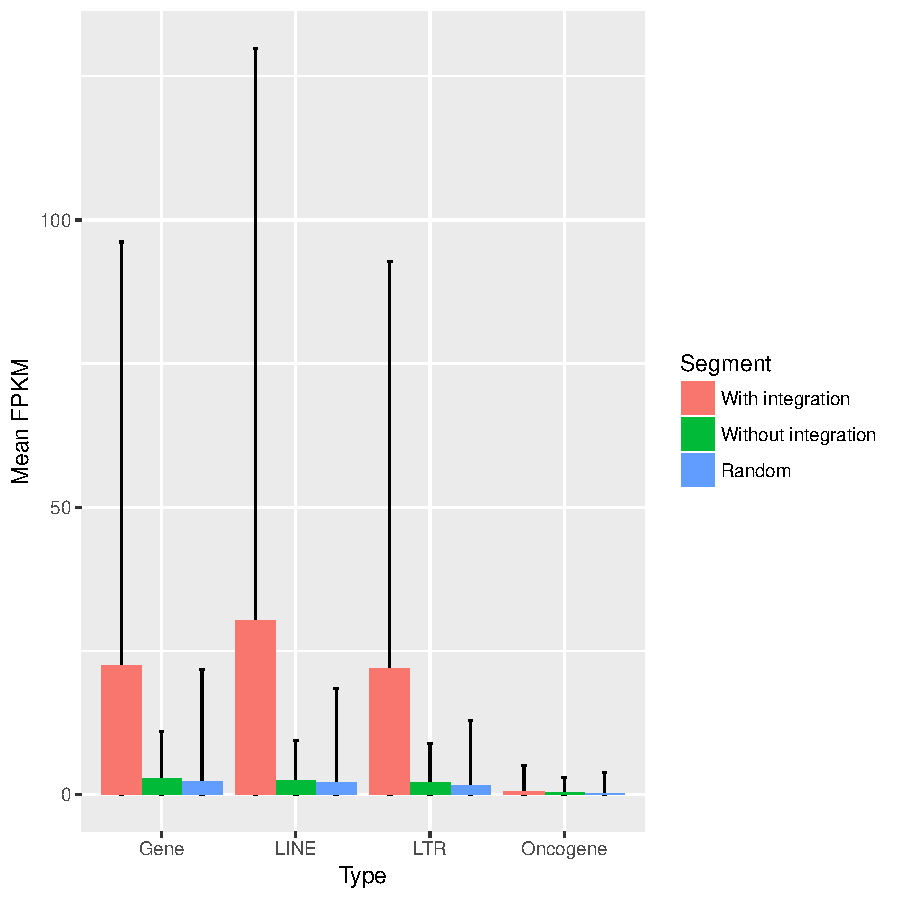
\includegraphics[width=1\linewidth]{{results/expression.summary.barplot}.pdf}\\
%\caption[Expression of mRNA transcripts in genomic segments with and without integrations.]
%{\label{expression_transcripts_fpkm}  {\bf Expression of mRNA transcripts in genomic segments with and without integrations.}  We report the mean FPKM expression of annotated features in genomic segments with and without integrations.  For a given integration in a sample, we select a 10kb flanking region around the integration site.  We then report the expression level in samples that have an integration in this region and samples that do not.  In addition, we report the expression level randomly selected segments as a baseline. The p-values for the paired Wilcoxon signed rank test of the difference in FPKM expression for genomic segments with and mean FPKM expression in segments without integrations are: LINE $<$ 1e-12;	LTR < 1e-10;  Gene < 1e-10; and	Oncogenes < NA.}
%\end{figure}

\begin{figure}[htpb]
  \centering
  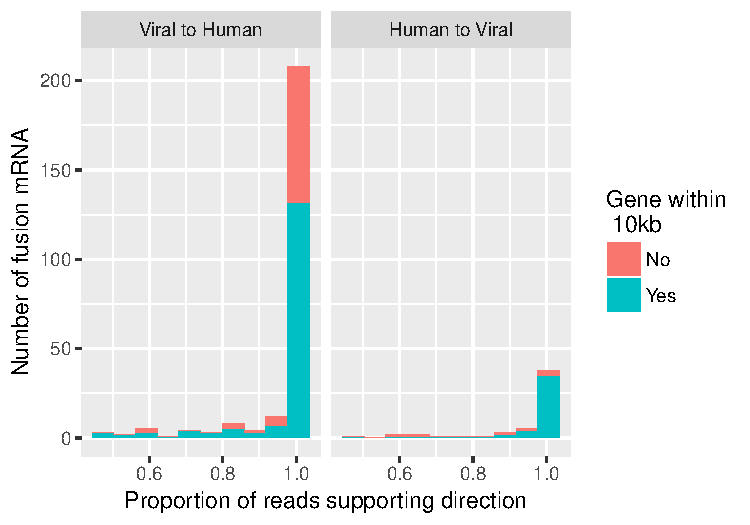
\includegraphics[width=1\linewidth]{{results/rna_direction.summary.histogram}.pdf}\\
\caption[Orientation of the mRNA fusion transcripts.]
{\label{mrna_directions}  {\bf Orientation of the mRNA fusion transcripts.}  We report whether the human portion of the fusion mRNA sequences are upstream or downstream of the viral portion.  The orientation is inferred from the paired-end reads under the assumption that the viral read is always oriented in the direction of the viral gene, and support for the orientation is computed as the proportion of paired-end reads supporting that orientation.  In addition, we report whether there is a gene within 10kb of the fusion mRNA read.}
\end{figure}

\begin{figure}[htpb]
 \centering
 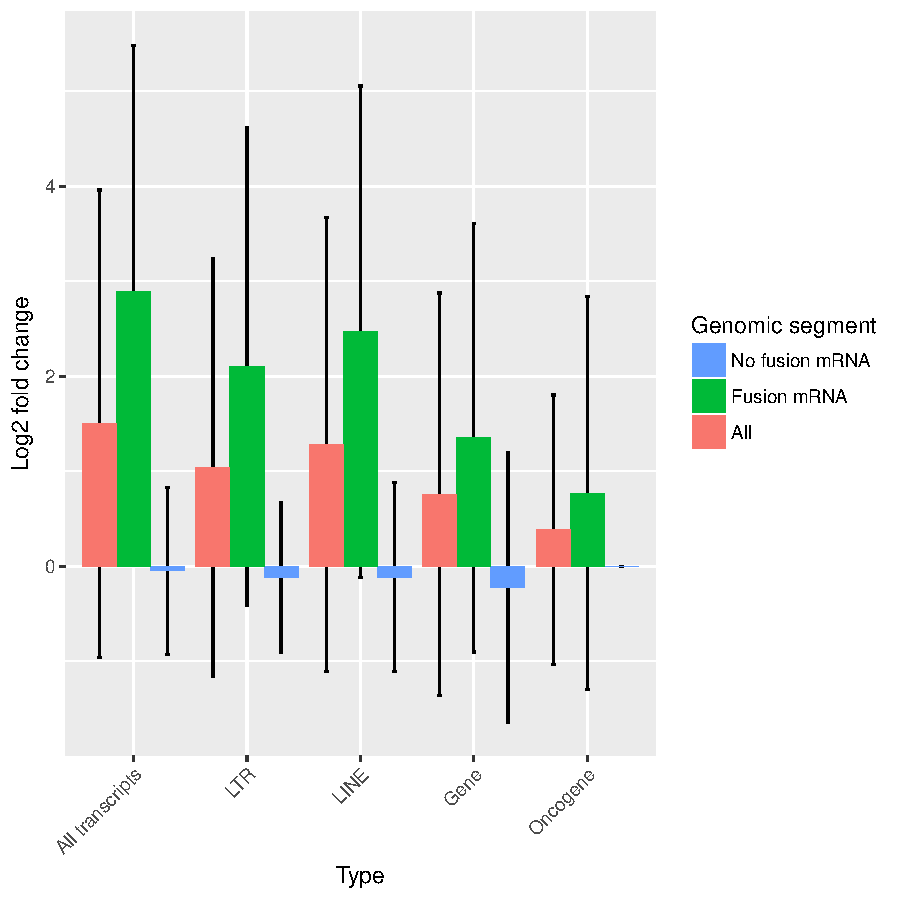
\includegraphics[ width=1\linewidth]{{results/expression.summary.barplot.fold}.pdf}\\
\caption[Expression of mRNA transcripts in genomic segments with and without integrations.]
{\label{expression_transcripts}  {\bf Log2 fold change in expression of mRNA transcripts in genomic segments with and without integrations.}  We report the Log2 fold change in expression of annotated features between genomic segments with and without integrations.  We report the average fold change for all segments, segments that contain fusion mRNA sequences, and segments without fusion mRNA sequences.  For a given integration in a sample, we select a 10kb flanking region around the integration site.  We then report the logfold change in expression level in samples that have an integration in this region and samples that do not.}
\end{figure}


\begin{figure}[htpb]
  \centering
  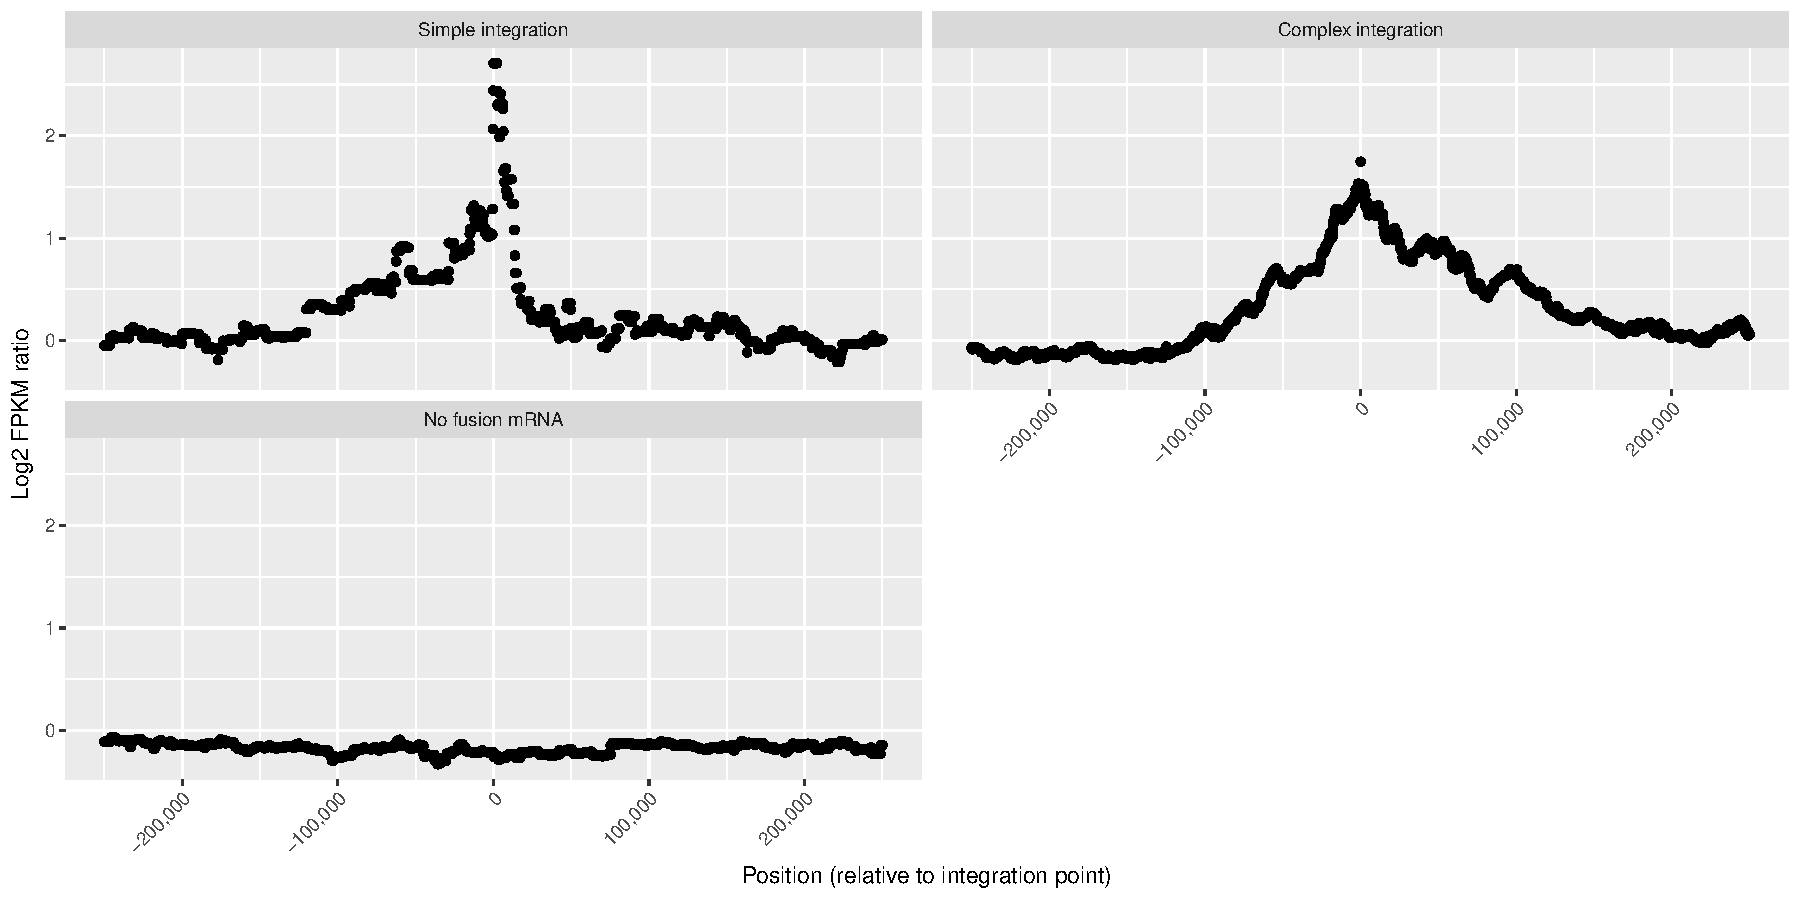
\includegraphics[width= 4in,frame]{{results/updown.250000}.pdf}
\caption[Fusion reads supp.]
{\label{updown_250kb}  {\bf Expression change around integration point within a 250kb window}.  We report the average log-fold expression change upstream and downstream of an integration event within a 250kb window.  The position is reported relative to the integration point in the human genome, with negative position being upstream of the integration event, and positive position being downstream of the integration event.  The results are separated out by the integration category. } %35, 110, 81
\end{figure}
\end{document}


\section*{Notes}

[1] N. Wentzensen, J. F. Coy, H. P. Knaebel, M. Linnebacher, B. Wilz, J. Gebert, and M. Von Knebel Doeberitz, “Expression of an endogenous retroviral sequence from the HERV-H group in gastrointestinal cancers,” Int. J. Cancer, vol. 121, no. 7, pp. 1417–1423, 2007.

Higher expression of HERV-H group in some cancers, not high in normal     

[1] M. T. Romanish, C. J. Cohen, and D. L. Mager, “Potential mechanisms of endogenous retroviral-mediated genomic instability in human cancer,” Semin. Cancer Biol., vol. 20, no. 4, pp. 246–253, 2010.

LTR and non-LTR not active, blocked by methalyation.  when meth. mech removed, the HERV become active.  

[1] A. Babaian and D. L. Mager, “Endogenous retroviral promoter exaptation in human cancer,” Mob. DNA, vol. 7, no. 1, p. 24, 2016.

LTR
Among them, pol is most conserved. Inside pol there are three important domains: IN(integrase), RT(reverse transcriptase) and RH(RNase H), which are enzymes for reverse transcription and insertion. RT and IN are regarded essential for autonomous LTR elements to fulfill their function.

LTR
no human LTRs transcriptionally active

Full length L1 have 2 internal promoters at 5' end, sense drives expression of element, antisense control transcription of nearby genes by forming chimeric transcripts, antisense promoter also express ORF0, which plays regulatory role in retrotransposition

500K L1, but only 3500-700 are full-length, retaining promoters




[1] M. Kadaja, A. Sumerina, T. Verst, M. Ojarand, E. Ustav, and M. Ustav, “Genomic instability of the host cell induced by the human papillomavirus replication machinery.,” EMBO J., vol. 26, no. 8, pp. 2180–91, 2007.

E1 protein is replicon origin recognition factor and viral helicase, which with E2, helps recruit(?) host cell replication complexes onto the HPV origin.  High E1 result in high recruitment of host replication complex at virus origin site.

Flanking DNA can be amplified, up to 12kb, with total amplicon size 25kb.  The amplification locus could be a target for genomic re-arrangments due to recruitment of DDR mechanisms.  In addition, onion-skin model of replication cuz breaks, fragments

[1] M. Kadaja, H. Isok-Paas, T. Laos, E. Ustav, and M. Ustav, “Mechanism of genomic instability in cells infected with the high-risk human papillomaviruses,” PLoS Pathog., vol. 5, no. 4, 2009.



[1] Z. Jiang, S. Jhunjhunwala, J. Liu, P. M. Haverty, M. I. Kennemer, Y. Guan, W. Lee, P. Carnevali, J. Stinson, S. Johnson, J. Diao, S. Yeung, A. Jubb, W. Ye, T. D. Wu, S. B. Kapadia, F. J. De Sauvage, R. C. Gentleman, H. M. Stern, S. Seshagiri, K. P. Pant, Z. Modrusan, D. G. Ballinger, and Z. Zhang, “The effects of hepatitis B virus integration into the genomes of hepatocellular carcinoma patients The effects of hepatitis B virus integration into the genomes of hepatocellular carcinoma patients,” pp. 593–601, 2012.

Runthrough for HBV, directional, need to make a clear graph
\section{Cell lines}
HPV16-positive W12 cell line both viral and integrated HPV genomes in early stages, lost of plasmids in later stages


%We examined the mean Fragments Per Kilobase of transcript per Million (FPKM) of genomic regions within 10kb of an integration compared to the mean FPKM of segments of samples without an integration in that region (Fig.~\ref{expression_transcripts}).  Genomic segments with integrations had increased expression of nearby human mRNA (2.5 fold increase), with significantly higher expression when human-viral fusion mRNA are present (5.5 fold increase).  Surprisingly, we found that integration also results in the expression of proximal LTR and LINE elements (3.5 to 5.3 fold increased expression when fusion mRNA is present).  


%and they have been implicated as causes in oncogenesis~\cite{Rodic2013,Xiao-Jie2016}.  While L1 elements are typically epigenetically repressed in  in germ and somatic cells,  , though this process is still poorly understood.  The integration process can create breaks in the host cell  genome, and it is hypothesized that and requires DNA repair mechanism to~\cite{Gasior2006,Rodic2013,Xiao-Jie2016}  
%
%LINE-1~\cite{Gasior2006}, and LINE L1 activity has been implicated in causing genomic instability and cancer~\cite{Rodic2013,Xiao-Jie2016}. 
%
%
%Hu et al. 2015 suggested that HPV may integrate randomly across the genome until an integration occurs in a region that provides a proliferation advantage and results in oncogenesis.  Thus, it's unsurprising to find that common regions with recurrent integrations are in or near known oncogenes. 
%
%~\cite{Tang2013,Hu2015}, and the second is identifying up-regulated or down-regulated host and viral genes resulting from integration~\cite{Tang2013}.  
%
% has highlighted genomic hotspots for integration, including known oncogenes such as MYC, PVT1, ERBB2, RAD51~\cite{Tang2013}, however, the vast majority of integrations are non-recurrent.  Hu et al. 2015 suggested that HPV may integrate randomly across the genome until an integration occurs in a region that provides a proliferation advantage and results in oncogenesis.  Thus, it's unsurprising to find that common regions with recurrent integrations are in or near known oncogenes.  
%
%Other research 



% short tandom repeats (STR), short interspersed nuclear element (SINE-Alu), long terminal repeat/endogenous retroviruses (LTR/ERV1), and Satellite
%For each integration, we examined the number of annotated genomic features within 10kb of the genomic integration(Fig.~\ref{integration_counts}) and compared the distribution of observed annotations to the expected annotations resulting from random intervals.  In particular, we focus on whether there is an enrichment of Long terminal repeats (LTR) and Long interspersed nuclear element (LINE) annotations near genomic integrations as these elements are typically not expressed in normal samples~\cite{Kinomoto2007,Sigurdsson2012}, but can be transcriptionally active in tumor samples~\cite{Romanish2010,Rodic2013,Xiao-Jie2016}.

%Previous research has observed that genomic regions with HPV integrations were enriched for genes~\cite{Akagi2014} or long terminal repeat/endogenous retroviruses (LTR/ERV1)~\cite{Hu2015} elements.  We also observed a significant enrichment of genes near integration points (Z-test; p-value $<$ 0.004).  We also detected a depletion of all LTR elements near integration points (Z-test; p-value $<$ 0.013), though after multiple hypothesis correction, this observation was not significant.  Finally, we detected a slight enrichment of oncogenes and no enrichment or depletion of LINE elements.  While many studies have noted that integrations do occur at or near oncogenes, these are very rare, and thus, can only explain tumorigenesis in the few cases in which they occur.  

%We observed recurrent integrations (within 50kb of each other) in two loci: two samples with integrations between region chr13:73955151-74005092 and four samples with integrations between region chr8:128747810-128889296.  The first region contains no nearby genes.  The latter region contains the MYC and PVT1 genes and had been found to contain recurrent integrations from previous studies~\cite{Hu2015}.  However, the vast majority of integrations are non-recurrent and occur uniquely within that particular sample, and thus, focusing on integrations that occur in genomic hotspots found across samples will exclude the majority of integrations and their roles on tumorigenesis.


%Details for each of the datasets is provided in the \textbf{Datasets} section, and a summary is provided in Table~\ref{table:data}. 



%Historically, viral integration was detected using PCR-based methods, however due to the labor intensive process of running the PCR experiments, and the low coverage and depth of PCR techniques, integration events were difficult to identify.  With the advent of Next Generation Sequencing (NGS) technology, human genomes can now be sequenced with high coverage and high sequencing depth thus making it more feasible to accurately identify the location of viral integrations within the human genome.  Many pipelines have been developed recently for the detection of viral integration from paired-end Illumina data (VirusSeq~\cite{Chen2013}, VirusFinder~\cite{Wang2013}, ViralFusionSeq~\cite{Li2013} in 2013; VERSE~\cite{Wang2015}, Virus-Clip~\cite{Ho2015}, and Vy-PER~\cite{Forster2015} in 2015).  While each pipeline varies in how detection is performed, the overarching theme is similar: identify single end or paired-end reads that map to both the human and viral reference genome.  Paired-end reads in which one read maps to a viral reference and the other read maps to a human reference (known as \emph{chimeric paired-end reads}) are indicative of a potential integration event.  Single end reads that partially map to a human reference and viral reference are known as \emph{split end reads} and are useful for determining the exact integration point in the human chromosome.  The key step for these methods is the use of a reference-based read mapper (i.e., BLAST~\cite{Altschul1990}, BLAT~\cite{Kent2002}, BowTie2~\cite{Langmead2012}, or BWA~\cite{Li2009}) to categorize the read pairs.  These methods perform pairwise sequence alignment between the query sequence and a reference sequence in order to determine if a) the query sequence is related to the reference, and b) the optimal alignment of the query sequence to the reference sequence.

%Integration can result in altered mRNA expression of flanking regions and viral-human fusion mRNA transcripts~\cite{Tang2013}.  Viral-human fusion transcripts can alter functional pathways, as in the case of the viral-human fusion transcript HBx-LINE1~\cite{Lau2014}, which acts as a sponge for miRNA-122 and promoted hepatic cell epithelial-mesenchymal transition (EMT)-like changes and increased susceptibility to induced tumor formation~\cite{Liang2016}.  

%Difficulties include the long latency period between infection and cancer formation (between 15 to 40 years for some cancers), the viruses that cause cancer in some patients often do not cause cancer in many other patients, and some viruses are indirect carcinogens (i.e., viral genes are not present in the tumor cells)~\cite{Hausen2009}.  Furthermore the human cancer viruses span across a diverse range of viral families, including retroviruses, positive-stranded RNA viruses, and small and large DNA viruses.  While these viral families have different cellular targets and different methods for proliferation, one key insight is that some of these viruses (Human papillomavirus (HPV), Molluscum contagiosum virus (MCV), Hepatitis B virus (HBV), and Human T-lymphotropic virus (HTLV)) have mechanisms for integrating directly into the host genome, and a tumor sample will show the same integration site throughout the sample, suggesting that integration occurred before clonal expansion of the tumor sample.  This observation suggests that integration may lead to cellular proliferation and cancer formation~\cite{Moore2010}.

%One challenge of reference-based pairwise alignment is in aligning reads from novel or evolutionarily divergent organisms~\cite{Brenner1998,Park1998}.  This can result in a poor alignment between the query sequence and the closest reference sequence or can even result in the failure to detect any evolutionary relationship between the query sequence and the known reference sequences.  An alternative approach is to first represent the relationships between the reference sequences using an evolutionary model.  Then a given query sequence can be scored against the model, and if the score is significant, fitted to the model.  One example of a commonly used evolutionary model is a \emph{profile Hidden Markov Model} (HMM;~\cite{Eddy1998}). HMMs are a statistical model for representing a multiple sequence alignment (MSA), and HMMs have been used to detect membership of query sequences to protein families~\cite{Finn2010}, align fragmentary sequences~\cite{Eddy1998}, and identify viral fragments from metagenomic samples~\cite{Skewes-Cox2014}.  Given a query sequence, the profile HMM can produce scores that represent the probability of the model generating the sequence, as well as the best alignment of the query sequence to the model.

%Previous research has shown that profile HMMs can have difficulty in recognizing sequences that come from evolutionarily divergent families, and that using an ensemble of profile HMMs (eHMMs) can improve recognition rates~\cite{Mirarab2012,Nguyen2014,Nguyen2015,Nguyen2016_hippi}.  The eHMMs technique has been shown to have better detection and alignment of query sequences to a given model compared to the single HMM approach, and as a result, better downstream downstream phylogenetic analyses. 

%We compare ViFi with VERSE~\cite{Wang2015} and ViralFusionSeq~\cite{Li2013} on both simulated and real biological datasets.  We selected VERSE and ViralFusionSeq for comparison as VERSE is among the most recent viral integration tools and has been shown to outperform VirusFinder and VirusSeq, and ViralFusionSeq is the only viral integration tool available on NIH HPC system.  We report the true positive and false positive integration points reported on the simulated datasets, and the true positive integration points reported on biological datasets with experimentally verified integration points.  Finally, we report the number of fusion transcripts detected from the matched RNA-seq datasets, and the number of those transcripts that are supported from the matched WGS datasets.

% (see Fig.~\ref{viral_discovery}).  The basic idea is to first map all paired end reads to both a human reference genome and to known viral reference genomes.  Second, paired end reads in which both reads map to the human reference are removed.  Third, paired end reads in which both reads map to viral genomes are used to identify potential viral candidates.  Fourth, for read pairs in which one read maps to a viral reference and the other read maps to a human reference (known as \emph{chimeric reads}) are indicative of a potential integration event.  Finally, in some cases, a single read might partially map to a human reference on one end and to the viral reference on another end.  These reads are known as \emph{split-end reads} and are useful for determining the exact integration point in the human chromosome.  The key step for these methods is the use of a reference-based read mapper (i.e., BLAST~\cite{Altschul1990}, BLAT~\cite{Kent2002}, BowTie2~\cite{Langmead2012}, or BWA~\cite{Li2009}) to categorize the read pairs.  These methods perform pairwise sequence alignment between the query sequence and a reference sequence in order to determine if a) the query sequence is related to the reference, and b) what is the optimal alignment of the query sequence to the reference sequence.
%For example, a recent study found recurrent HPV integrations in several oncogenes~\cite{Hu2015}.  The authors hypothesized that HPV might first integrate randomly across the genome, however over the long term, integrations at key loci may provide a selective advantage to the host cells, resulting in hot-spots genes with recurrent integration.  Another HPV study found that more than half of HPV-infected tumors had viral-human fusion transcripts, suggesting that the host-spot locations are transcriptionally active~\cite{Schmitz2012}.  In many cases, integrated HPV genomes have a disrupted E2 gene; the suppression of the viral E2 gene can result in suppression of the tumor suppressor p53 gene in humans~\cite{Akagi2014}. Another recent study found that copy number variations (CNV) were significantly increased near HBV integration locations which the authors suggest that integration may cause chromosomal instability~\cite{Sung2012}.  In addition, the authors found recurrent integration in or near several oncogenes, including TERT, which produces an enzyme that is found in high activity in cancer cells.  Thus, being able to identify integration locations can help us detect hotspot genes with recurrent integrations, identify fusion transcript, find oncoproducts, and examine the chromosomal stability around the integration point.  All of these factors can help us better understand the mechanisms of how a normal cell might transform into a tumor cell upon infection.


%\begin{figure}[htpb]
%  \centering
%  \includegraphics[width=1\linewidth]{{viral_discovery_1}.pdf}\\
%\caption[paired end sequencing viral integration discovery pipeline.]
%{\label{viral_discovery}  {\bf Viral integration and discovery.}  1) The human genome (represented in blue) has a viral integration event (represented in red).  2) The DNA is extracted and fragmented.  Some fragments will consist of only human DNA, some fragments will consist of viral DNA, and some fragments will be chimeric.  3) The fragments are sequenced via Illumina paired end sequencing technology and mapped to onto a human reference and a viral reference.  3) Depending on which reference(s) the paired end reads map onto, pairs are grouped into four categories: a) human, b) viral, c) chimeric, or d) split.}
%\end{figure}

%\begin{figure}[htpb]
%  \centering
%  
\includegraphics[width=0.75\linewidth]{{results/fusion_TCGA-C5-A0TN}.pdf}\\
%  \caption[Example of fusion mRNA found by ViFi.] {{\bf Example of fusion mRNA found by ViFi  \label{vifi_exmaple}}  We show an example of a fusion mRNA event found by ViFi that was not reported by the Tang et al. 2014 study nor found by VERSE for the sample TCGA-C5-A0TN on the genomic segment chr3:126,847,238-126,849,346.  The first track is the results from mapping the RNA-seq data, and the second track is the results from mapping the WGS data.  Reads in red are chimeric reads in which one end maps to the human hg19 reference (shown) and the other end maps to the viral reference.  The results show that both the top and bottom track contain chimeric reads clustered around this interval.}
%\end{figure}
